% ===========================================================
% บทที่ 4: ผลการทดลองและอภิปรายผล
% ===========================================================

บทนี้นำเสนอผลตามลำดับที่ทำจริง เริ่มจากการปรับจูนและการเลือก Checkpoint
ตามด้วยผลบนชุดทดสอบ ผลของ Diffusion ความเห็นของผู้ใช้ เหตุผลที่เลือกโมเดลไปใช้บนเว็บ
และผลการใช้งานเว็บจริง ท้ายบทเป็นการอภิปรายว่าผลเหล่านี้บอกอะไร
เพื่อให้อ่านง่าย บทนี้ใช้ตัวย่อดังนี้ HFG คือ HairFastGAN, BS คือ Barbershop ก่อนปรับจูน,
BS-FT หรือ Barbershop-FT คือ Barbershop ที่ปรับจูนแล้ว (Fine-tuned), B24 คือ Trial B Epoch 24,
A30 คือ Trial A Epoch 30 และ Diff คือขั้นขัดเกลาด้วย Diffusion

% -----------------------------------------------------------
\section{ผลการปรับจูนและการเลือก Checkpoint}
% -----------------------------------------------------------

\subsection{ตัวอย่างการคำนวณค่าสูญเสีย}

ก่อนดูผลการเลือก ผู้วิจัยขอแสดงตัวอย่างว่าค่าสูญเสียในบทที่ 3 คำนวณออกมาเป็นตัวเลขอย่างไร
ตารางที่~\ref{tab:loss_example} ใช้ HFG Trial B เป็นตัวอย่าง โดยเทียบ Epoch 0 (ก่อนฝึก) กับ Epoch 24 (ตัวที่ถูกเลือก)
ทุกค่าเป็นค่าเฉลี่ยบนชุดตรวจสอบ 9 ชุด คอลัมน์ ``น้ำหนัก'' คือตัวคูณตามสมการที่~(\ref{eq:loss}) และ~(\ref{eq:loss_hfg})
คอลัมน์ Epoch 0 และ Epoch 24 คือค่าก่อนคูณ และคอลัมน์ ``$\times$ น้ำหนัก'' คือค่าหลังคูณ
ซึ่งรวมกันได้ค่าในแถวสุดท้าย (0.6183 และ 0.3957) ตรงกับค่าที่บันทึกไว้ระหว่างการฝึก

ตารางนี้บอกได้มากกว่าตัวเลขรวม ถ้าดูคอลัมน์หลังคูณน้ำหนัก จะเห็นว่าที่ Epoch 0
สองด้านที่มีค่ามากที่สุดคือบริเวณที่ต้องคงเดิม (0.194) และสีผม (0.141) ซึ่งตรงกับปัญหาใบหน้าซีดและสีเป็นปื้นที่เห็นด้วยตา
หลังฝึก สองด้านนี้ก็ลดลงมากที่สุด (เหลือ 0.085 และ 0.073) ส่วนทรงผมลดลงเพียงเล็กน้อย
ซึ่งเป็นไปตามที่คาด เพราะโมดูลที่ควบคุมทรงถูกล็อกไว้
ค่าสูญเสียยึดรหัส (Anchor) เป็น 0 ที่ Epoch 0 เพราะยังไม่มีอะไรเปลี่ยน และเพิ่มขึ้นเล็กน้อยเมื่อโมเดลเริ่มเปลี่ยน

\begin{table}[!htbp]
\centering
\caption{ค่าสูญเสียแยกแต่ละส่วนของ HFG Trial B (ค่าเฉลี่ยชุดตรวจสอบ)}
\label{tab:loss_example}
\begin{tabular}{|l|c|c|c|c|c|}
\hline
\textbf{ส่วนของค่าสูญเสีย} & \textbf{น้ำหนัก} & \textbf{Epoch 0} & \textbf{$\times$ น้ำหนัก}
& \textbf{Epoch 24} & \textbf{$\times$ น้ำหนัก} \\ \hline
$L_{color}$ & 1.0 & 0.1412 & 0.1412 & 0.0732 & 0.0732 \\ \hline
$L_{shape}$ & 0.2 & 0.4590 & 0.0918 & 0.4263 & 0.0853 \\ \hline
$L_{id}$ & 0.1 & 0.2523 & 0.0252 & 0.1945 & 0.0194 \\ \hline
$L_{protect}$ & 5.0 & 0.0387 & 0.1936 & 0.0170 & 0.0851 \\ \hline
$L_{detail}$ & 0.1 & 0.5816 & 0.0582 & 0.5009 & 0.0501 \\ \hline
$L_{color}(I_{pre})$ & 0.5 & 0.1280 & 0.0640 & 0.0778 & 0.0389 \\ \hline
$L_{shape}(I_{pre})$ & 0.1 & 0.4428 & 0.0443 & 0.4122 & 0.0412 \\ \hline
Anchor & 0.01 & 0.0000 & 0.0000 & 0.2556 & 0.0026 \\ \hline
\textbf{รวม} & & & \textbf{0.6183} & & \textbf{0.3957} \\ \hline
\end{tabular}
\par\vspace{3pt}{\footnotesize\raggedright หมายเหตุ: HFG = HairFastGAN\par}

\end{table}

ลองคำนวณบางส่วนด้วยมือ เช่น $L_{color}$ ที่ Epoch 0 มี $E_L = 8.053$ และ $E_{ab} = 6.071$
จึงได้ $L_{color} = (8.053 + 6.071)/100 = 0.1412$
และ $L_{id}$ มีค่าโคไซน์ของ ArcFace (Additive Angular Margin Loss) เท่ากับ 0.7477 จึงได้ $L_{id} = 1 - 0.7477 = 0.2523$
สำหรับ BS-FT Trial A ซึ่งไม่มีส่วนที่วัดภาพกลาง ค่ารวมที่ Epoch 0 คือ
$0.1501 + 0.2 \times 0.4432 + 0.1 \times 0.2554 + 5 \times 0.0373 + 0.1 \times 0 = 0.4508$
และลดลงเหลือ 0.4036 ที่ Epoch 30 ซึ่งลดลงน้อยกว่า HFG มาก สาเหตุจะเห็นชัดในหัวข้อถัดไป

\subsection{HairFastGAN: เลือก Trial B Epoch 24}

ตารางที่~\ref{tab:select_hfg} สรุป Checkpoint ที่ดีที่สุดของแต่ละ Trial ของ HFG
คอลัมน์ ``Epoch ที่ดีที่สุด'' คือ Epoch ที่คะแนนต่ำสุดใน Trial นั้น
คอลัมน์ ``คะแนน'' คิดตามสมการที่~(\ref{eq:score}) และคอลัมน์สุดท้ายคือจำนวน Epoch ที่ผ่านครบ 5 ด่าน
สิ่งที่น่าพอใจของ HFG คือทุก Trial ผ่านด่านครบทุก Epoch แปลว่าการปรับจูนไม่ได้ทำให้ด้านอื่นแย่ลงเลย
การตัดสินจึงขึ้นกับคะแนนเพียงอย่างเดียว และ Trial B Epoch 24 ได้คะแนนดีที่สุดคือ 0.664
แม้จะต่างจาก Trial A เพียง 0.023 แต่ผู้วิจัยยึดตามกติกาที่ตั้งไว้ ไม่เลือกตามความชอบ
คะแนนของ B24 คำนวณได้ดังนี้
\begin{equation}
\text{score} = \frac{1}{2}\left(\frac{7.32}{14.12} + \frac{1 - 0.924}{1 - 0.906}\right)
= \frac{1}{2}\left(0.518 + 0.810\right) = 0.664
\label{eq:score_example}
\end{equation}
\begin{vardef}
7.32, 14.12 & สีผิดเฉลี่ยที่ Epoch 24 และที่ Epoch 0 \\
0.924, 0.906 & IoU เฉลี่ยที่ Epoch 24 และที่ Epoch 0 \\
0.518, 0.810 & สัดส่วนสีผิดและทรงผิดเทียบกับตอนก่อนฝึก
\end{vardef}
แปลว่าความผิดพลาดของสีและทรงโดยเฉลี่ยเหลือร้อยละ 66.4 ของตอนก่อนฝึก
แต่ถ้าแยกดูจะเห็นว่าสีผิดลดลงเกือบครึ่ง (เหลือ 0.518) ขณะที่ทรงผิดลดลงไม่ถึงหนึ่งในห้า (เหลือ 0.810)
คะแนนที่ดีขึ้นส่วนใหญ่จึงมาจากเรื่องสี

\begin{table}[!htbp]
\centering
\caption{ผลการเลือก Checkpoint ของ HairFastGAN (ชุดตรวจสอบ 9 ชุด)}
\label{tab:select_hfg}
\begin{tabular}{|c|c|c|c|}
\hline
\textbf{Trial} & \textbf{Epoch ที่ดีที่สุด} & \textbf{คะแนน} & \textbf{Epoch ที่ผ่าน 5 ด่าน} \\ \hline
A & 27 & 0.687 & 30/30 \\ \hline
\textbf{B} & \textbf{24} & \textbf{0.664} & 30/30 \\ \hline
C & 26 & 0.712 & 30/30 \\ \hline
D & 23 & 0.716 & 30/30 \\ \hline
\end{tabular}
\end{table}

ภาพที่~\ref{fig:select_hfg} แสดงว่าคะแนนเปลี่ยนไปอย่างไรตลอด 30 Epoch
แกนนอนคือ Epoch แกนตั้งคือคะแนน (ยิ่งต่ำยิ่งดี) เส้นประด้านบนคือระดับ 1.00 ของ Epoch 0
เส้นสีส้มเข้มคือ Trial B ที่ถูกเลือก เส้นสีเทาคืออีกสาม Trial และจุดที่มีกรอบคือ Epoch 24
สิ่งแรกที่เห็นคือทุก Trial ดีขึ้นเร็วมากในช่วง 5 Epoch แรก หลังจากนั้นคะแนนแกว่งขึ้นลง ส่วนใหญ่อยู่ระหว่าง 0.70--0.82
(ต่ำสุด 0.664 ที่ B24 และมีบางจุดขึ้นไปถึงประมาณ 0.90)
ไม่ได้ลดลงเรื่อย ๆ อย่างที่อาจคาดไว้ การแกว่งนี้ส่วนหนึ่งเป็นเพราะชุดตรวจสอบมีเพียง 9 ชุด
ภาพเดียวที่ดีขึ้นหรือแย่ลงก็ทำให้ค่าเฉลี่ยกระโดดได้
นี่คือเหตุผลที่ต้องตั้งกติกาไว้ล่วงหน้า ถ้าดูกราฟแล้วเลือกด้วยตา อาจเลือกได้หลายจุดและอธิบายไม่ได้ว่าทำไม

\begin{figure}[!htbp]
\centering
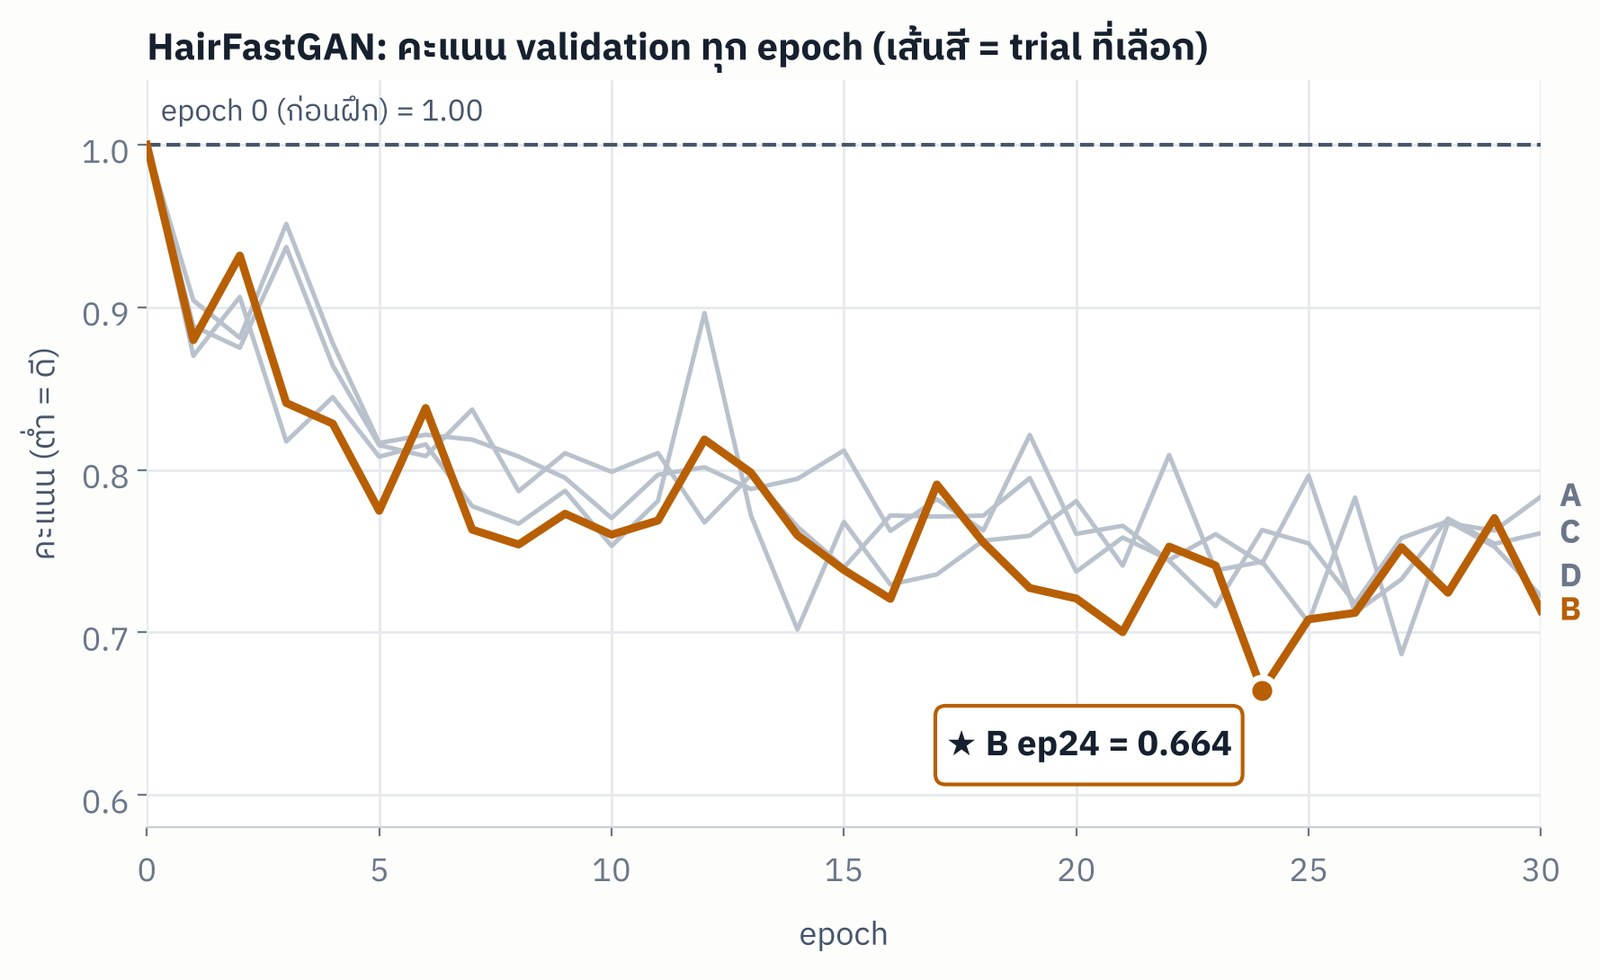
\includegraphics[width=0.85\textwidth]{images/01_select_hfg.jpg}
\caption{คะแนนบนชุดตรวจสอบทุก Epoch ของ HairFastGAN (เส้นสีคือ Trial B ที่เลือก)}
\label{fig:select_hfg}
\par\vspace{3pt}{\footnotesize\raggedright หมายเหตุ: HFG = HairFastGAN, B24 = น้ำหนักของ Trial B Epoch 24, ep = Epoch\par}
\end{figure}

คะแนนดูเพียงสีกับทรง ภาพที่~\ref{fig:5m_hfg} จึงแยกออกเป็น 5 กราฟเพื่อดูทุกด้านพร้อมกัน
แต่ละกราฟมีแกนนอนเป็น Epoch แกนตั้งเป็นค่าของตัวชี้วัด และเส้นสีแต่ละเส้นคือหนึ่ง Trial
เส้นประสีเทาคือค่าที่ Epoch 0 ส่วนเส้นประสีแดงกับพื้นสีแดงจางคือเขตที่ไม่ผ่านด่าน
จุดคือ Checkpoint ที่เลือก และใต้ชื่อกราฟเขียนเกณฑ์ของด่าน พร้อมค่าก่อนและหลังของ B24 ไว้

ภาพนี้ยืนยันว่า HFG ดีขึ้นทุกด้านพร้อมกัน ไม่ได้แลกด้านหนึ่งกับอีกด้านหนึ่ง
ที่ B24 สีผิดลดจาก 14.12 เหลือ 7.32 IoU (Intersection over Union) เพิ่มจาก 0.906 เป็น 0.924
ArcFace เพิ่มจาก 0.748 เป็น 0.806 MAE (Mean Absolute Error) ของบริเวณที่ต้องคงเดิมลดจาก 0.039 เหลือ 0.017
และค่ารายละเอียดผมลดจาก 0.61 เหลือ 0.52 ทุกเส้นอยู่ฝั่งที่ผ่านด่านตลอด
(ค่ารายละเอียดผมในกราฟนี้คือค่าที่ระบบบันทึกตอนตรวจด่านที่ 5 ซึ่งบันทึกแยกจากค่า $L_{detail}$ ในตารางที่~\ref{tab:loss_example} ตัวเลขจึงไม่เท่ากันพอดี)
ที่น่าสนใจคือ ArcFace และ MAE ดีขึ้นอย่างสม่ำเสมอ เส้นเรียบและไม่ค่อยแกว่ง
ขณะที่เส้นสีผิดแกว่งมากที่สุด แปลว่าโมดูล Refinement เรียนเรื่องใบหน้าได้ง่ายและนิ่ง
ส่วนเรื่องสีขึ้นกับภาพแต่ละชุดมากกว่า

\begin{figure}[!htbp]
\centering
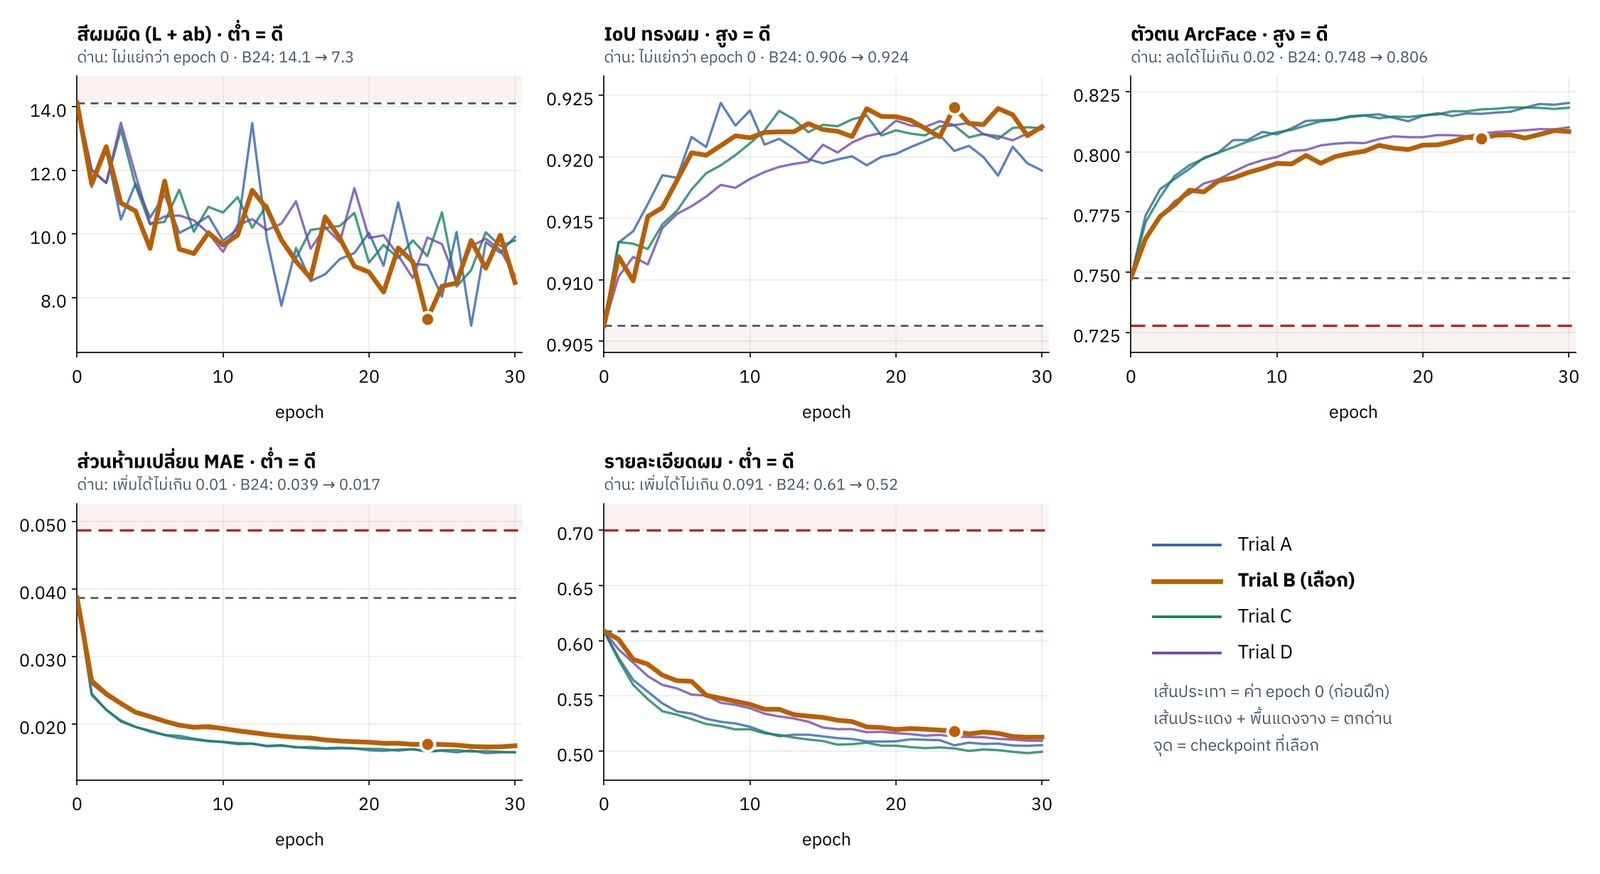
\includegraphics[width=\textwidth]{images/fig_5m_hfg.jpg}
\caption{ตัวชี้วัด 5 ด้านบนชุดตรวจสอบทุก Epoch ของ HairFastGAN ทั้ง 4 Trial}
\label{fig:5m_hfg}
\par\vspace{3pt}{\footnotesize\raggedright หมายเหตุ: IoU = Intersection over Union (สัดส่วนพื้นที่ผมที่ทับกัน), MAE = Mean Absolute Error (ค่าความคลาดเคลื่อนสัมบูรณ์เฉลี่ย), ArcFace = โมเดลจดจำใบหน้าที่ใช้วัดความเหมือนของใบหน้า, HFG = HairFastGAN\par}
\end{figure}

\subsection{Barbershop-FT: เลือก Trial A Epoch 30}

การเลือกของ Barbershop-FT ซับซ้อนกว่า ตารางที่~\ref{tab:select_bs} แสดงผลที่ Epoch 30 ของแต่ละ Trial
คอลัมน์ ``ผล'' บอกว่าผ่านครบ 5 ด่านหรือไม่ผ่านด่านใด และคอลัมน์สุดท้ายคือจำนวน Epoch ที่ผ่านครบ
ต่างจาก HFG ตรงที่ BS-FT มีหลาย Epoch ที่ไม่ผ่านด่าน และด่านที่เป็นปัญหาคือด่านทรงผม
Trial C และ D มี IoU ต่ำกว่าตอนก่อนฝึกทุก Epoch จึงไม่มีสิทธิ์ถูกเลือกเลย
ส่วน Trial A และ B เพิ่งผ่านในช่วงท้ายของการฝึก

ตรงนี้มีข้อจำกัดที่ผู้วิจัยต้องยอมรับ ระหว่างฝึก BS-FT ระบบวัดผลทุก Epoch ก็จริง
แต่บันทึกไฟล์น้ำหนักไว้เพียง Epoch 0 และ 30 ตัวเลือกที่ใช้ได้จริงจึงมีเพียง Epoch 30
ซึ่ง Trial A ได้คะแนนดีที่สุดคือ 0.841
ถ้าบันทึกไว้ครบทุก Epoch ตัวที่ดีที่สุดจะเป็น Trial B Epoch 29 (0.840)
แต่ต่างกันเพียง 0.001 และไม่มีไฟล์ให้ใช้ ผู้วิจัยจึงใช้ A30

\begin{table}[!htbp]
\centering
\caption{ผลการเลือก Checkpoint ของ Barbershop-FT ที่ Epoch 30 (ชุดตรวจสอบ 9 ชุด)}
\label{tab:select_bs}
\begin{tabular}{|c|c|c|c|}
\hline
\textbf{Trial} & \textbf{คะแนน Epoch 30} & \textbf{ผล} & \textbf{Epoch ที่ผ่าน 5 ด่าน} \\ \hline
\textbf{A} & \textbf{0.841} & ผ่านครบ & 13/30 \\ \hline
B & 0.842 & ผ่านครบ & 8/30 \\ \hline
C & 0.856 & ตกด่านทรง & 0/30 \\ \hline
D & 0.858 & ตกด่านทรง & 0/30 \\ \hline
\end{tabular}
\par\vspace{3pt}{\footnotesize\raggedright หมายเหตุ: BS-FT (Barbershop-FT) = Barbershop ที่ปรับจูนแล้ว (Fine-tuned)\par}

\end{table}

ภาพที่~\ref{fig:select_bs} อ่านแบบเดียวกับภาพที่~\ref{fig:select_hfg} โดยเส้นสีน้ำเงินเข้มคือ Trial A
ลักษณะของกราฟต่างจาก HFG อย่างชัดเจน คะแนนลดลงต่อเนื่องและเรียบกว่ามาก
เพราะ BS-FT ฝึกบนรหัสชุดเดิมที่เก็บไว้ ข้อมูลที่โมเดลเห็นจึงไม่เปลี่ยน
แต่ลดลงได้น้อยกว่า HFG มาก โดยไปหยุดที่ประมาณ 0.84 เทียบกับ 0.66 ของ HFG
สาเหตุคือทรงผมของ BS-FT ถูกกำหนดเสร็จตั้งแต่ขั้นจัดรูป ก่อนถึงชั้นที่ปรับจูน
ครึ่งหนึ่งของคะแนน (ส่วนทรง) จึงแทบขยับไม่ได้

\begin{figure}[!htbp]
\centering
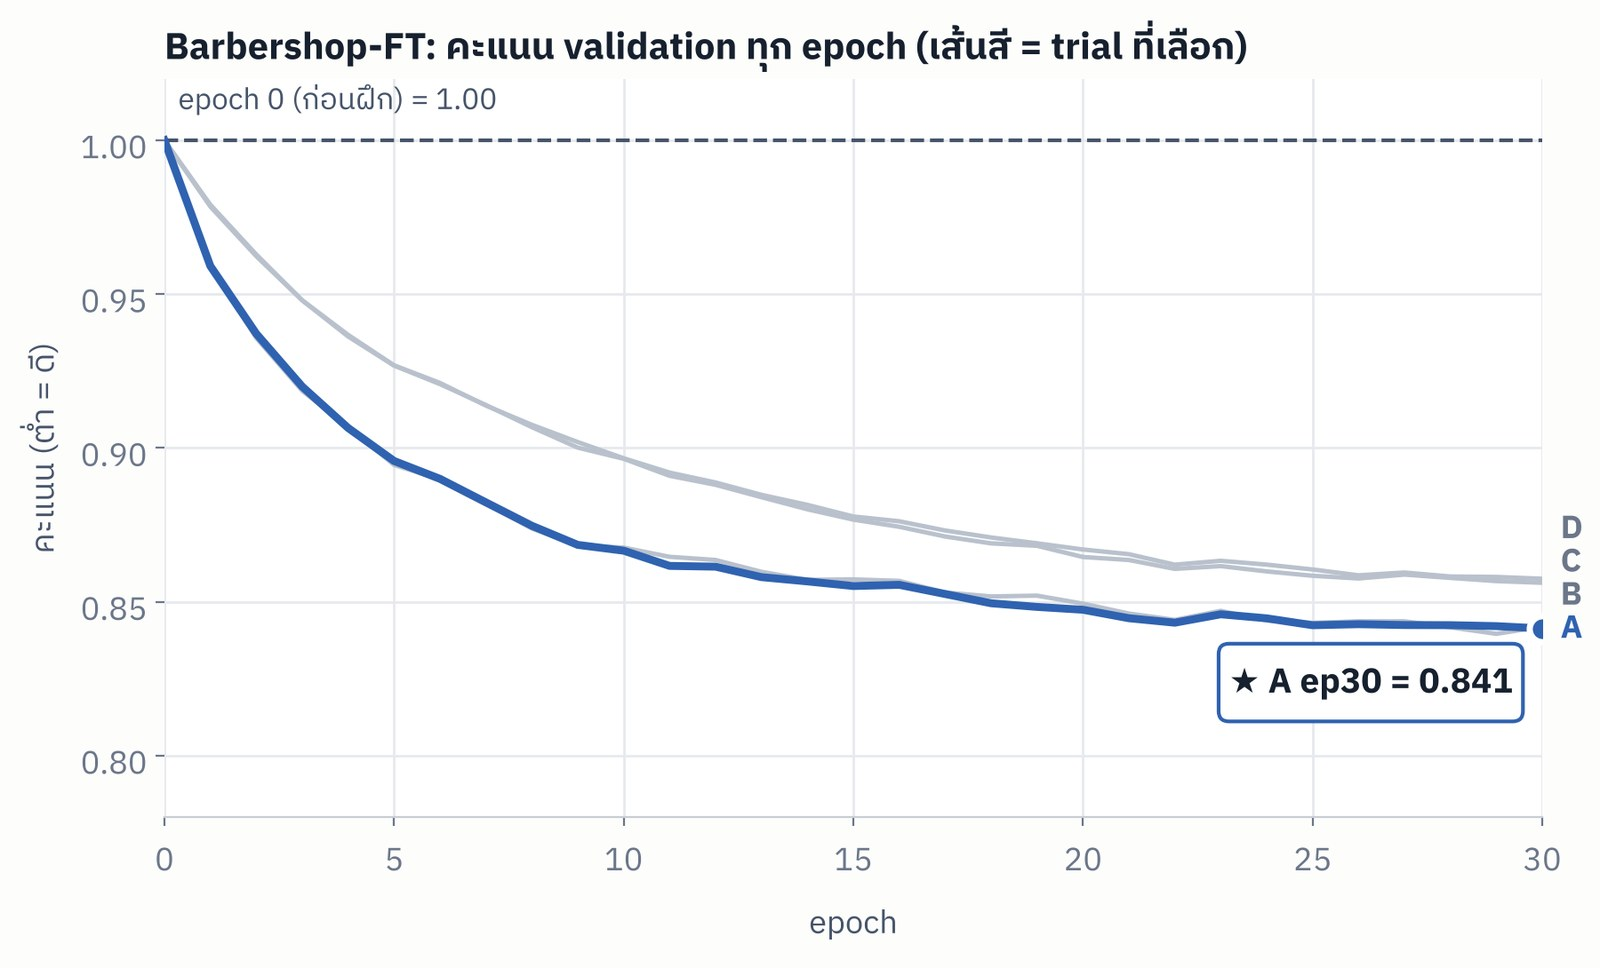
\includegraphics[width=0.85\textwidth]{images/02_select_bs.jpg}
\caption{คะแนนบนชุดตรวจสอบทุก Epoch ของ Barbershop-FT (เส้นสีคือ Trial A ที่เลือก)}
\label{fig:select_bs}
\par\vspace{3pt}{\footnotesize\raggedright หมายเหตุ: BS-FT (Barbershop-FT) = Barbershop ที่ปรับจูนแล้ว (Fine-tuned), A30 = น้ำหนักของ Trial A Epoch 30, ep = Epoch\par}
\end{figure}

ภาพที่~\ref{fig:5m_bs} แยกดูทั้ง 5 ด้านของ BS-FT แบบเดียวกับภาพที่~\ref{fig:5m_hfg}
ที่ A30 สีผิดลดจาก 15.0 เหลือ 10.3 ArcFace เพิ่มจาก 0.745 เป็น 0.748
MAE ลดจาก 0.037 เหลือ 0.036 และค่ารายละเอียดผมเพิ่มจาก 0 เป็น 0.07 ซึ่งยังอยู่ในขอบ 0.091
กราฟที่ควรดูมากที่สุดคือกราฟ IoU เส้นของ Trial C และ D (สีเขียวและสีม่วง) อยู่ในพื้นที่สีแดงตลอด
ส่วน Trial A ค่อย ๆ ไต่ขึ้นมาเหนือเส้นประสีเทาหลัง Epoch ที่ 17 และจบที่ 0.8973
กราฟนี้แสดงว่าอัตราการเรียนรู้ของกลุ่มแรกมีผลกับทรงผม
Trial C และ D ใช้อัตราการเรียนรู้กลุ่มแรกที่ต่ำกว่า และไม่เคยดึงทรงกลับขึ้นมาได้

\begin{figure}[!htbp]
\centering
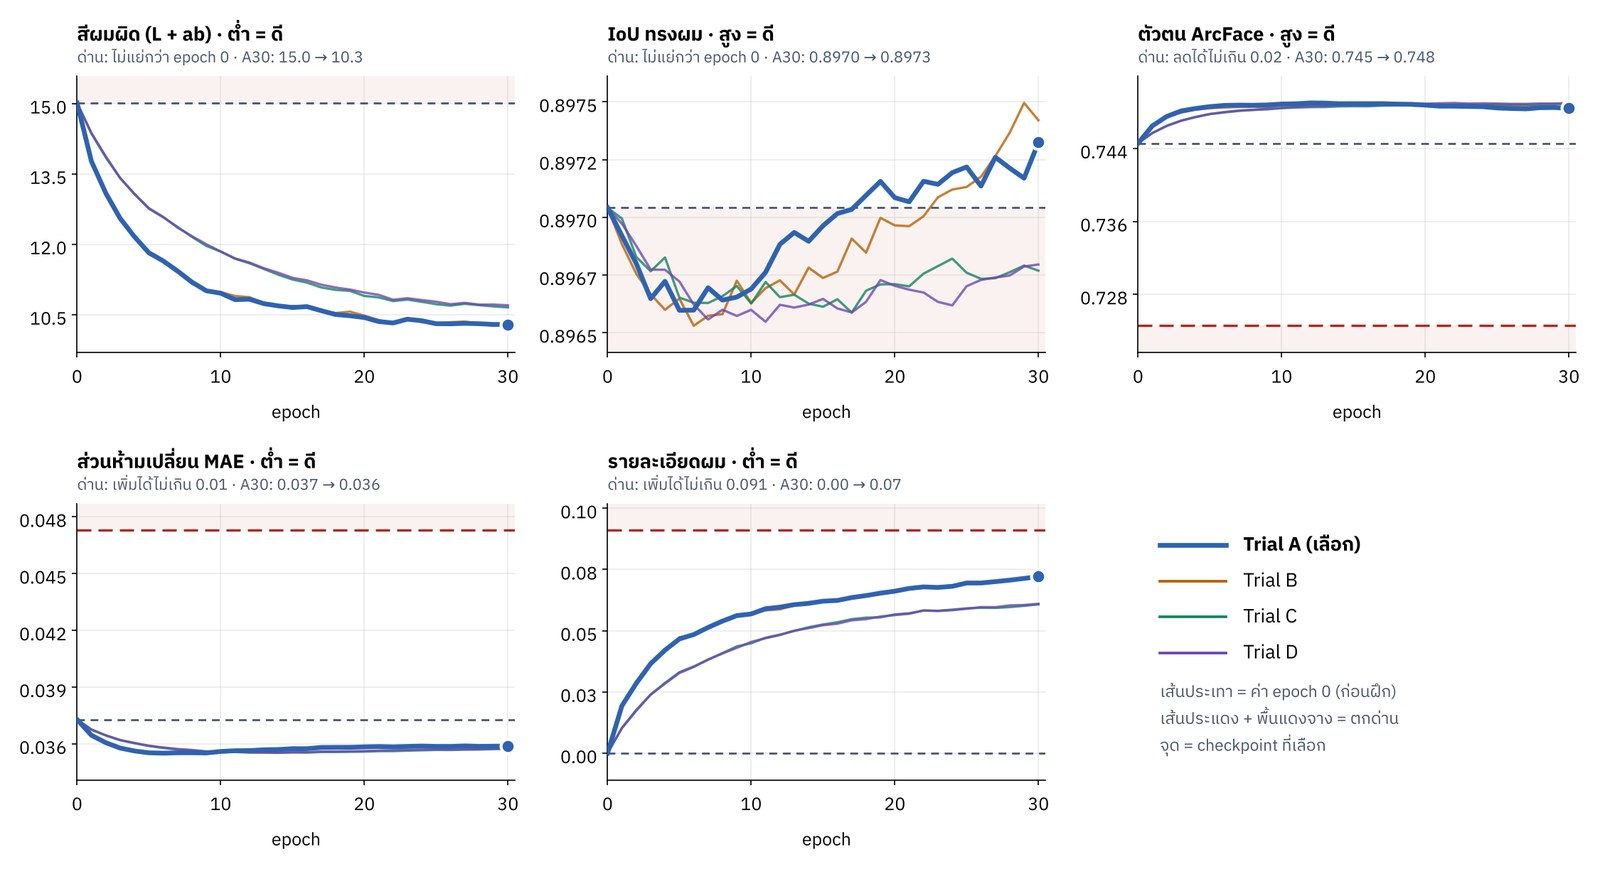
\includegraphics[width=\textwidth]{images/fig_5m_bs.jpg}
\caption{ตัวชี้วัด 5 ด้านบนชุดตรวจสอบทุก Epoch ของ Barbershop-FT ทั้ง 4 Trial}
\label{fig:5m_bs}
\par\vspace{3pt}{\footnotesize\raggedright หมายเหตุ: BS-FT (Barbershop-FT) = Barbershop ที่ปรับจูนแล้ว (Fine-tuned), IoU = Intersection over Union (สัดส่วนพื้นที่ผมที่ทับกัน), MAE = Mean Absolute Error (ค่าความคลาดเคลื่อนสัมบูรณ์เฉลี่ย), ArcFace = โมเดลจดจำใบหน้าที่ใช้วัดความเหมือนของใบหน้า\par}
\end{figure}

% -----------------------------------------------------------
\section{ผลบนชุดทดสอบ}
% -----------------------------------------------------------

หัวข้อนี้เป็นผลการวัด Checkpoint ที่เลือกบนชุดทดสอบ 10 ชุด หลังจากล็อกตัวเลือกแล้ว ซึ่งเป็นตัวเลขที่ผู้วิจัยให้น้ำหนักมากที่สุด
ทั้งนี้ ผู้วิจัยเคยประเมินโมเดลก่อนปรับจูน (Baseline) บนชุดนี้ไปแล้วครั้งหนึ่งก่อนแก้กติกาการเลือก ตามที่เปิดเผยไว้ในบทที่ 3
ตารางที่~\ref{tab:test} แสดงค่าเฉลี่ยก่อนและหลังปรับจูนของแต่ละโมเดลในคอลัมน์ที่สองและสาม
ลูกศรหลังชื่อตัวชี้วัดบอกทิศทางที่ดี ($\downarrow$ ต่ำ = ดี, $\uparrow$ สูง = ดี)
คอลัมน์ที่สี่คือผลต่างแบบจับคู่ของ BS-FT ลบ BS พร้อมช่วงความเชื่อมั่น 95\%
และคอลัมน์สุดท้ายคือข้อสรุป คำว่า ``ชัด'' หมายถึงช่วงความเชื่อมั่นไม่ครอบคลุมเลข 0

ผลบนชุดทดสอบไปในทางเดียวกับชุดตรวจสอบ คือการปรับจูนช่วยทั้งสองโมเดล
HFG B24 ดีขึ้นมากด้านใบหน้า (ArcFace จาก 0.728 เป็น 0.794) และบริเวณที่ต้องคงเดิม (MAE ลดลงเกือบสามเท่า)
ส่วน BS-FT A30 ดีขึ้นน้อยกว่าในทุกด้าน แต่ให้สีผมใกล้เป้าหมายที่สุดในตาราง (7.86)
ประเด็นที่ไม่ควรมองข้ามคือเวลา HFG ใช้ประมาณ 10 วินาที ส่วน BS ใช้ประมาณ 657 วินาที หรือเกือบ 11 นาที

\begin{table}[!htbp]
\centering
\caption{ผลบนชุดทดสอบ 10 ชุด (ค่าเฉลี่ย) และผลต่างแบบจับคู่ของ Barbershop}
\label{tab:test}
\footnotesize
\begin{tabular}{|l|c|c|c|c|}
\hline
\textbf{ตัวชี้วัด} & \textbf{HFG ก่อน $\rightarrow$ B24} & \textbf{BS ก่อน $\rightarrow$ FT A30}
& \textbf{BS-FT $-$ BS (95\% CI)} & \textbf{สรุป BS} \\ \hline
สีผิด $\downarrow$ & 13.03 $\rightarrow$ 8.99 & 8.77 $\rightarrow$ 7.86 & $-0.91$ ($-3.54$ ถึง $+1.90$) & ยังไม่ชัด \\ \hline
IoU ทรง $\uparrow$ & 0.904 $\rightarrow$ 0.920 & 0.885 $\rightarrow$ 0.888 & $+0.003$ ($+0.000$ ถึง $+0.006$) & เล็กน้อย \\ \hline
ArcFace $\uparrow$ & 0.728 $\rightarrow$ 0.794 & 0.711 $\rightarrow$ 0.724 & $+0.013$ ($+0.008$ ถึง $+0.019$) & ชัด \\ \hline
MAE $\downarrow$ & 0.041 $\rightarrow$ 0.014 & 0.036 $\rightarrow$ 0.033 & $-0.003$ ($-0.004$ ถึง $-0.001$) & ชัด \\ \hline
SSIM $\uparrow$ & 0.904 $\rightarrow$ 0.947 & 0.899 $\rightarrow$ 0.911 & $+0.012$ ($+0.008$ ถึง $+0.015$) & ชัด \\ \hline
เวลาต่อภาพ $\downarrow$ & ประมาณ 10 วินาที & ประมาณ 657 วินาที & -- & -- \\ \hline
\end{tabular}
\par\vspace{3pt}{\footnotesize\raggedright หมายเหตุ: HFG = HairFastGAN, B24 = น้ำหนักของ Trial B Epoch 24, BS = Barbershop ก่อนปรับจูน, BS-FT (Barbershop-FT) = Barbershop ที่ปรับจูนแล้ว (Fine-tuned), A30 = น้ำหนักของ Trial A Epoch 30, CI = Confidence Interval (ช่วงความเชื่อมั่น), IoU = Intersection over Union (สัดส่วนพื้นที่ผมที่ทับกัน), ArcFace = โมเดลจดจำใบหน้าที่ใช้วัดความเหมือนของใบหน้า, MAE = Mean Absolute Error (ค่าความคลาดเคลื่อนสัมบูรณ์เฉลี่ย), SSIM = Structural Similarity Index (ดัชนีความคล้ายเชิงโครงสร้าง)\par}

\end{table}

ค่าเฉลี่ยของ 10 ภาพอาจถูกดึงขึ้นหรือลงด้วยภาพเดียวได้ ภาพที่~\ref{fig:test_metrics} จึงแสดงผลรายภาพ
แต่ละกราฟมี 4 แถวคือ 4 ระบบ (HFG ก่อนฝึก, HFG B24, BS ก่อนฝึก และ BS-FT A30)
จุดจางแต่ละจุดคือภาพทดสอบหนึ่งภาพ ขีดเข้มคือค่าเฉลี่ย เส้นประเชื่อมค่าเฉลี่ยก่อนและหลังปรับจูน
และข้อความด้านขวาบอกว่าดีขึ้นกี่ภาพจาก 10 ภาพ

เมื่อดูรายภาพ ผลของ HFG น่าเชื่อถือขึ้นมาก เพราะ ArcFace, MAE และ SSIM (Structural Similarity Index) ดีขึ้นครบ 10 จาก 10 ภาพ
แปลว่าค่าเฉลี่ยไม่ได้ถูกดึงขึ้นด้วยภาพเพียงไม่กี่ภาพ แต่ดีขึ้นทุกภาพจริง
ช่วงความเชื่อมั่นของ IoU ($+0.016$; $+0.003$ ถึง $+0.033$), ArcFace ($+0.066$; $+0.051$ ถึง $+0.082$),
MAE ($-0.027$) และ SSIM ($+0.043$) ไม่ครอบคลุมเลข 0 ทั้งหมด
ที่ยังไม่ชัดคือสี แม้สีผิดลดลงเฉลี่ย 4.04 แต่ช่วงความเชื่อมั่นยังแตะ 0 ($-8.19$ ถึง $+0.30$)
เพราะมี 3 ภาพที่สีแย่ลง จึงยังสรุปไม่ได้ว่าการปรับจูนแก้เรื่องสีได้ทุกกรณี
สำหรับ BS-FT ArcFace และ SSIM ดีขึ้นครบ 10 จาก 10 ภาพเช่นกัน MAE ดีขึ้น 8 ภาพ และสีดีขึ้น 7 ภาพ
แม้ขนาดของการเปลี่ยนแปลงจะเล็ก แต่ทิศทางสม่ำเสมอ

\begin{figure}[!htbp]
\centering
\begin{subfigure}{\textwidth}
\centering
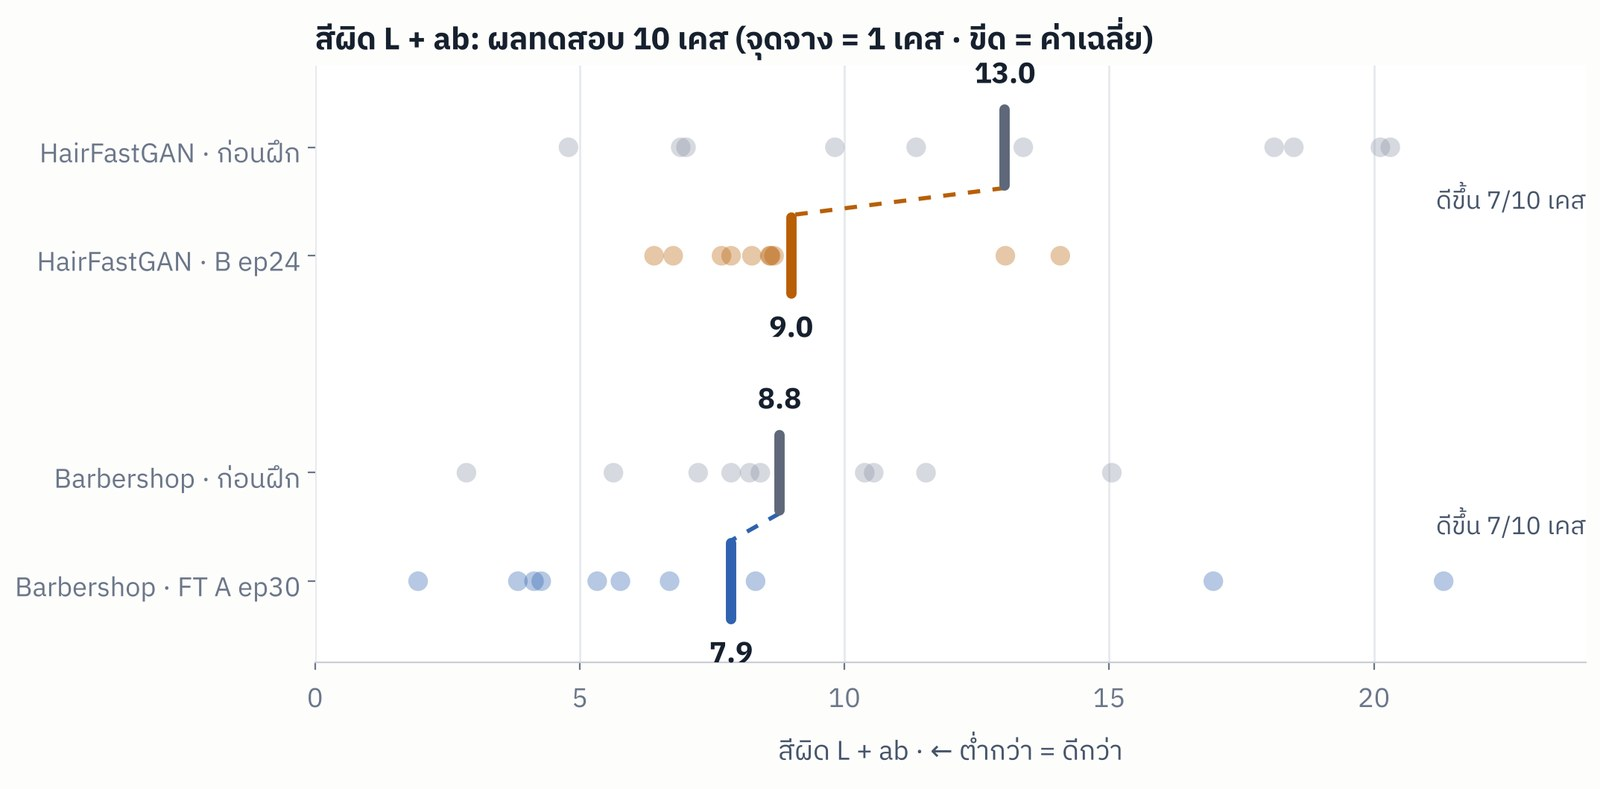
\includegraphics[width=0.74\textwidth]{images/03_test_color.jpg}
\caption{สีผิด}
\end{subfigure}
\vspace{0.3em}
\begin{subfigure}{\textwidth}
\centering
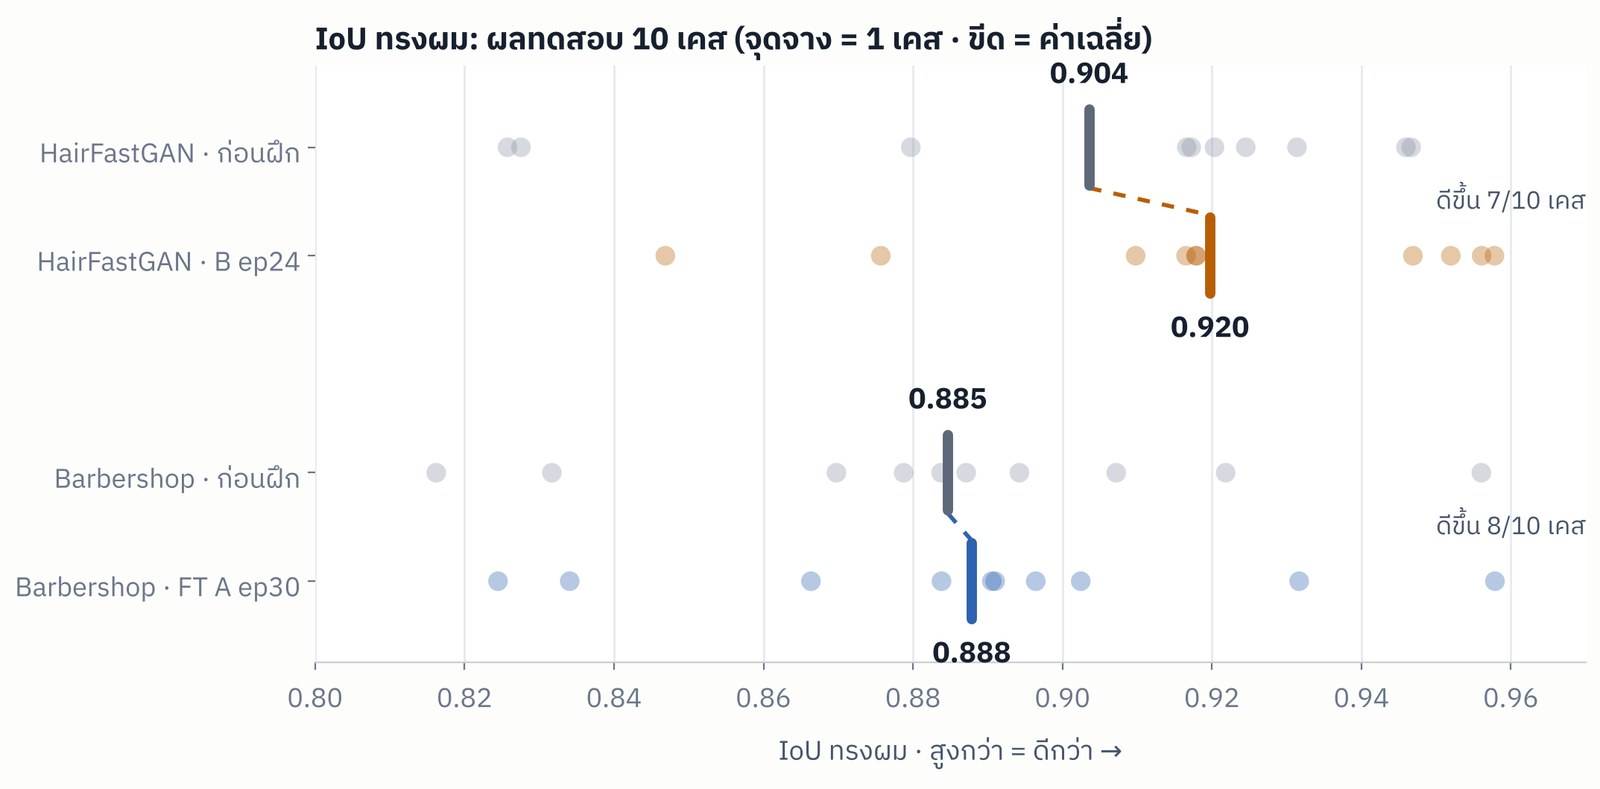
\includegraphics[width=0.74\textwidth]{images/04_test_iou.jpg}
\caption{IoU ทรงผม}
\end{subfigure}
\vspace{0.3em}
\begin{subfigure}{\textwidth}
\centering
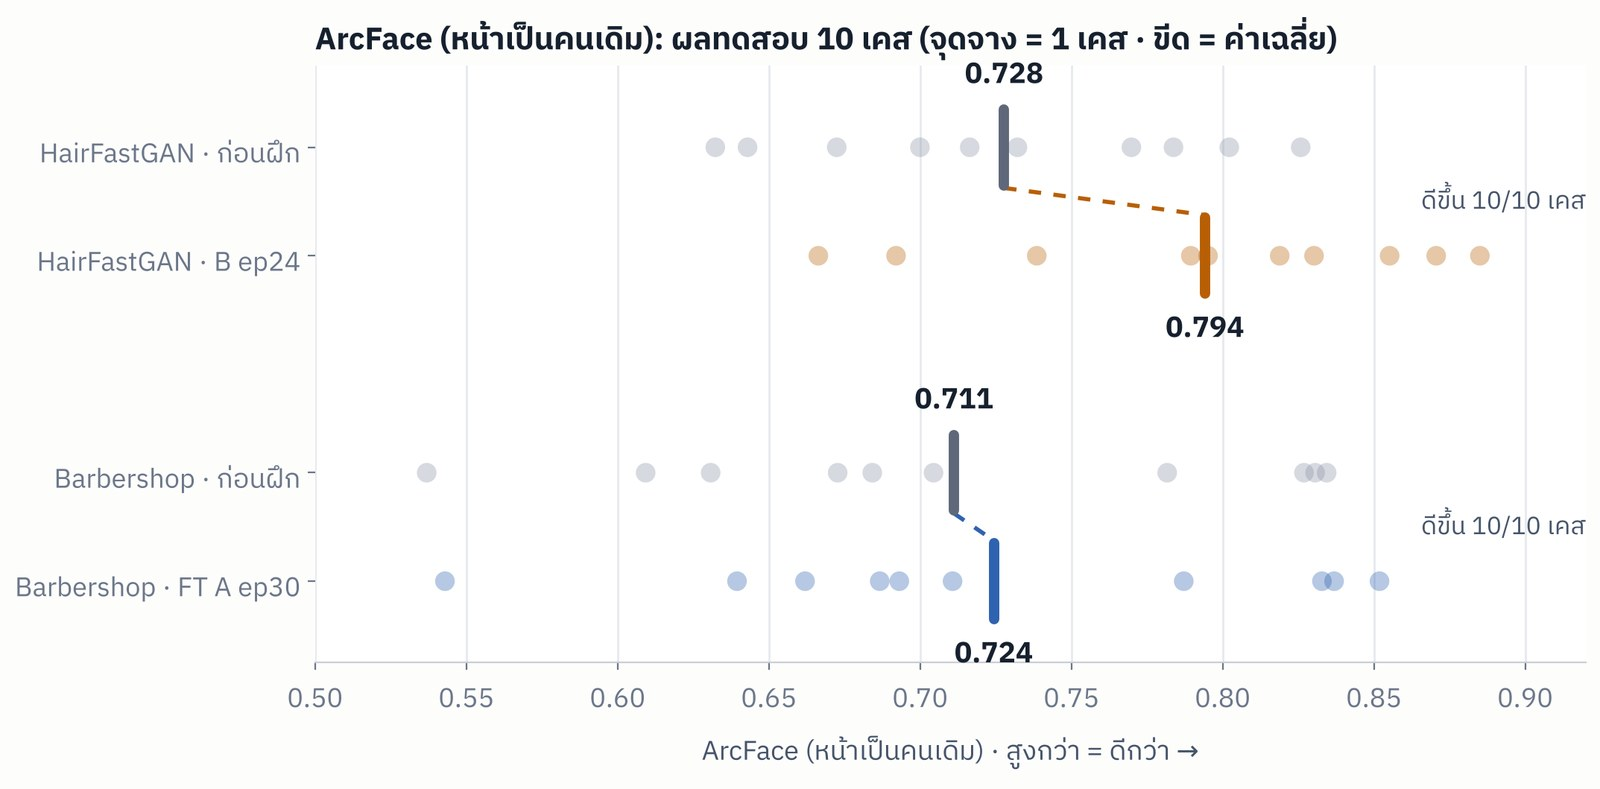
\includegraphics[width=0.74\textwidth]{images/05_test_arcface.jpg}
\caption{ArcFace}
\end{subfigure}
\caption{ผลบนชุดทดสอบรายภาพ (จุดจาง = 1 ภาพ, ขีดเข้ม = ค่าเฉลี่ย)}
\label{fig:test_metrics}
\par\vspace{3pt}{\footnotesize\raggedright หมายเหตุ: IoU = Intersection over Union (สัดส่วนพื้นที่ผมที่ทับกัน), ArcFace = โมเดลจดจำใบหน้าที่ใช้วัดความเหมือนของใบหน้า, MAE = Mean Absolute Error (ค่าความคลาดเคลื่อนสัมบูรณ์เฉลี่ย), SSIM = Structural Similarity Index (ดัชนีความคล้ายเชิงโครงสร้าง), HFG = HairFastGAN, BS = Barbershop ก่อนปรับจูน, BS-FT (Barbershop-FT) = Barbershop ที่ปรับจูนแล้ว (Fine-tuned), B24 = น้ำหนักของ Trial B Epoch 24, ep = Epoch, A30 = น้ำหนักของ Trial A Epoch 30\par}
\end{figure}

\begin{figure}[!htbp]
\ContinuedFloat
\centering
\begin{subfigure}{\textwidth}
\centering
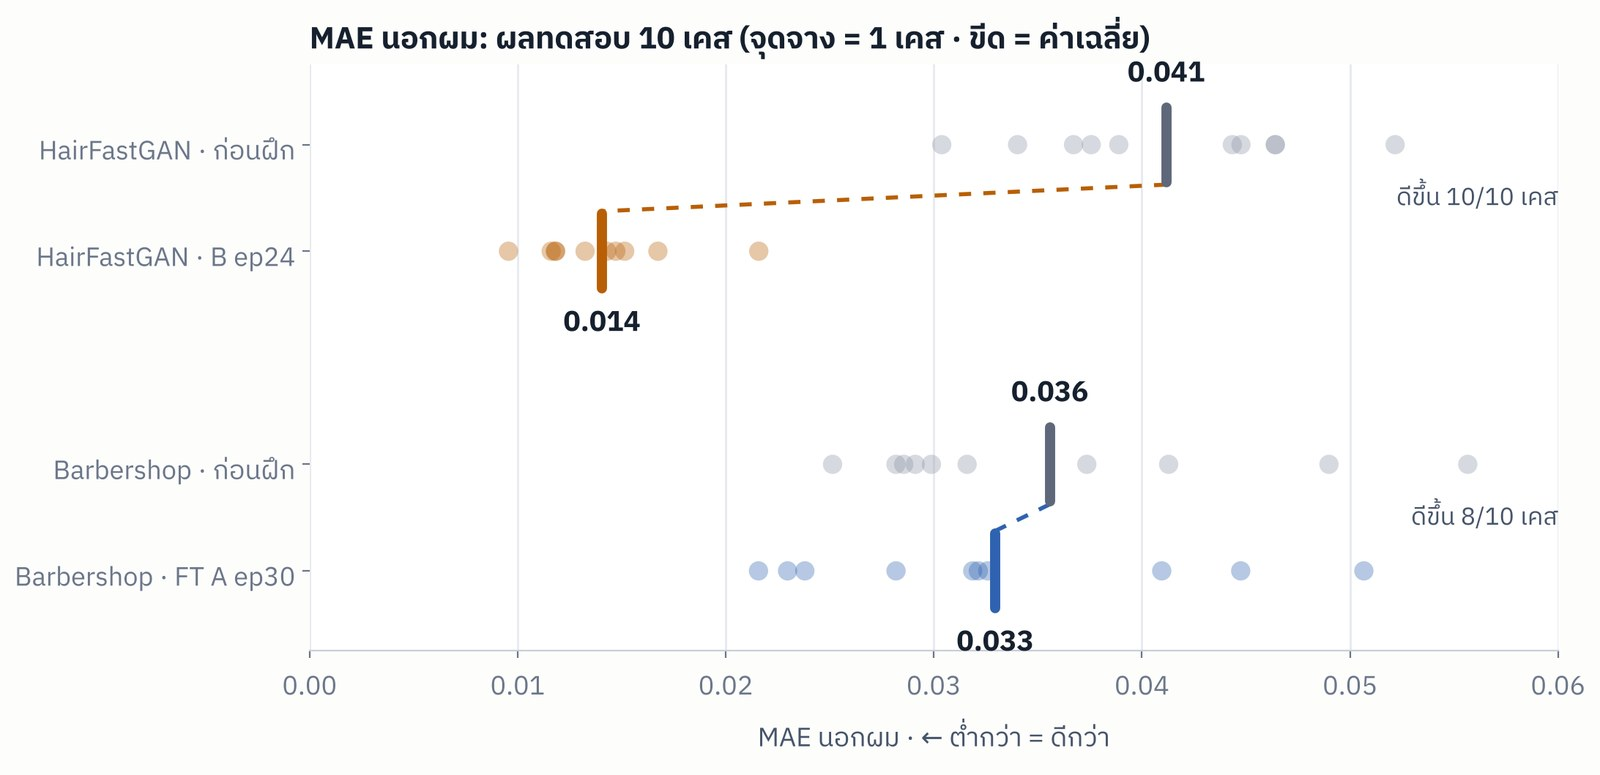
\includegraphics[width=0.82\textwidth]{images/06_test_mae.jpg}
\caption{MAE นอกผม}
\end{subfigure}
\vspace{0.3em}
\begin{subfigure}{\textwidth}
\centering
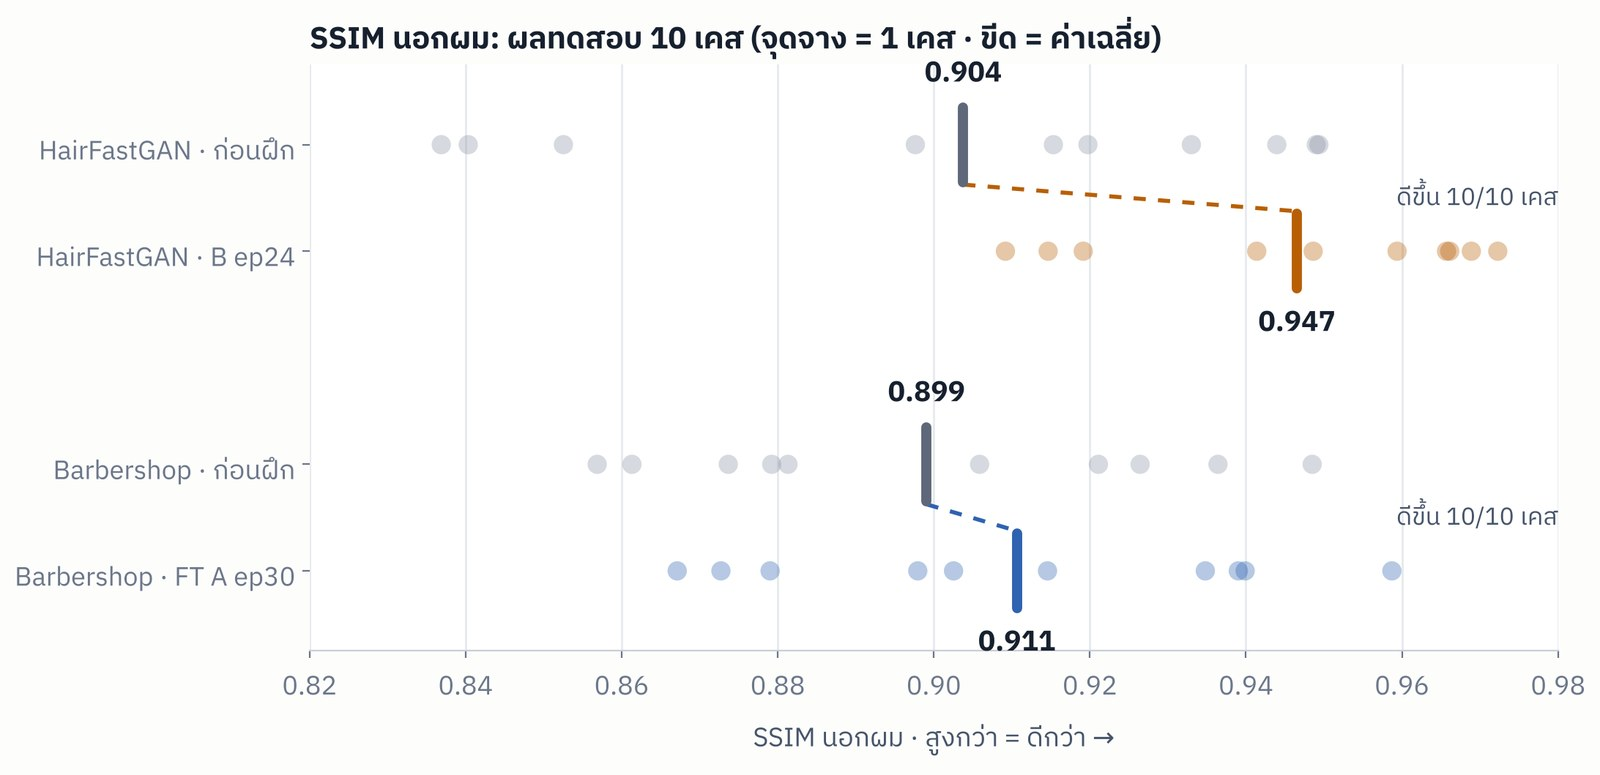
\includegraphics[width=0.82\textwidth]{images/07_test_ssim.jpg}
\caption{SSIM นอกผม}
\end{subfigure}
\caption[]{ผลบนชุดทดสอบรายภาพ (ต่อ)}
\par\vspace{3pt}{\footnotesize\raggedright หมายเหตุ: IoU = Intersection over Union (สัดส่วนพื้นที่ผมที่ทับกัน), ArcFace = โมเดลจดจำใบหน้าที่ใช้วัดความเหมือนของใบหน้า, MAE = Mean Absolute Error (ค่าความคลาดเคลื่อนสัมบูรณ์เฉลี่ย), SSIM = Structural Similarity Index (ดัชนีความคล้ายเชิงโครงสร้าง), HFG = HairFastGAN, BS = Barbershop ก่อนปรับจูน, BS-FT (Barbershop-FT) = Barbershop ที่ปรับจูนแล้ว (Fine-tuned), B24 = น้ำหนักของ Trial B Epoch 24, ep = Epoch, A30 = น้ำหนักของ Trial A Epoch 30\par}
\end{figure}

ตัวเลขทั้งหมดข้างต้นจะเข้าใจง่ายขึ้นเมื่อดูภาพจริง ภาพที่~\ref{fig:test_case} คือชุดทดสอบ test\_000
แถวบนคือภาพนำเข้า (ใบหน้า ทรงผม และสีผม) และแถวล่างคือผลของ 4 ระบบ
เรียงจากซ้ายไปขวาเป็น HFG ก่อนฝึก, HFG B24, BS ก่อนฝึก และ BS-FT A30
ถ้าเทียบสองภาพแรกจะเห็นปัญหาที่กล่าวถึงตั้งแต่บทที่ 1 คือ HFG ก่อนปรับจูนให้ผมเป็นปื้นที่สีไม่สม่ำเสมอ
หลังปรับจูนสีกลืนกันมากขึ้นและใกล้ภาพอ้างอิงขึ้น
ส่วนคู่ของ Barbershop สีดีขึ้นเล็กน้อย แต่ทรงผมแทบเหมือนเดิม ในบางภาพผมยังขาดเป็นช่วง หรือไม่เข้ากับรูปหน้า
ซึ่งเป็นผลโดยตรงจากการที่ทรงถูกกำหนดก่อนถึงชั้นที่ปรับจูน

\begin{figure}[!htbp]
\centering
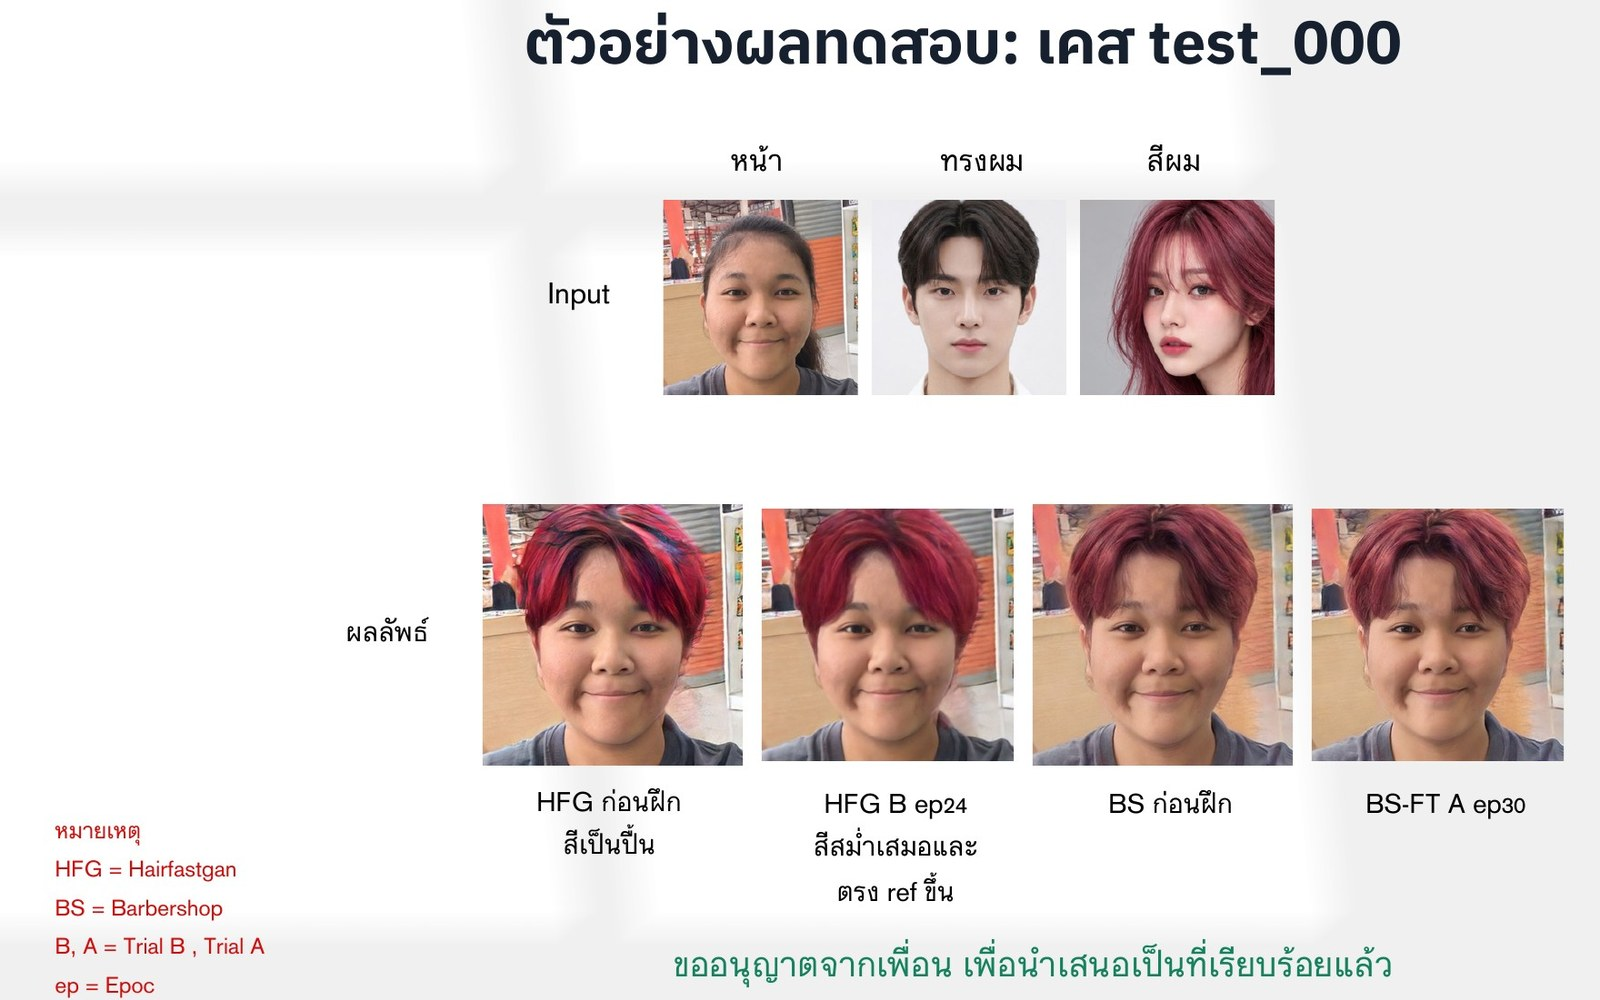
\includegraphics[width=0.85\textwidth]{images/fig_test_case.jpg}
\caption{ตัวอย่างผลบนชุดทดสอบ (test\_000) ของโมเดลก่อนและหลังปรับจูน}
\label{fig:test_case}
\par\vspace{3pt}{\footnotesize\raggedright หมายเหตุ: HFG = HairFastGAN, BS = Barbershop ก่อนปรับจูน, BS-FT (Barbershop-FT) = Barbershop ที่ปรับจูนแล้ว (Fine-tuned), B24 = น้ำหนักของ Trial B Epoch 24, ep = Epoch, A30 = น้ำหนักของ Trial A Epoch 30\par}
\end{figure}

% -----------------------------------------------------------
\section{ผลของขั้นขัดเกลาด้วย Diffusion}
\label{sec:diff_result}
% -----------------------------------------------------------

สิ่งที่ตาเห็นต้องตรวจสอบด้วยตัวเลขด้วย ผู้วิจัยจึงรันกรณีศึกษา 8 ชุดภาพ แต่ละชุดประกอบด้วยภาพใบหน้า ภาพทรงผม และภาพสีผม
รวมใบหน้า 7 คน (ชุดที่ 1 และ 6 เป็นคนเดียวกันแต่ใช้ทรงและสีต่างกัน)
แล้วสร้างภาพด้วย HFG B24 และ BS-FT A30 (Barbershop-FT Trial A Epoch 30) ซึ่งเป็นสองโมเดลที่ใช้ในแบบสอบถาม
จากนั้นขัดเกลาด้วยค่าเดียวกันทุกอย่าง (Seed 3407, Strength 0.15, 30 ขั้น, CFG 2.5) และวัดผลหลังแต่ละขั้น
ผู้วิจัยรันไว้ทั้งหมด 9 ชุด แต่ขั้นวัดผลของชุดสุดท้ายทำงานไม่เสร็จ จึงไม่นำมาคิด
ภาพที่~\ref{fig:diff_cases} แสดงตัวอย่าง 2 ชุดจาก 8 ชุด ในแต่ละชุด แถวบนคือ BS-FT A30 และแถวล่างคือ HFG B24
จากซ้ายไปขวาคือ ก่อน Diffusion, หลัง Diffusion, หลังเก็บพื้นหลัง และหลัง Native Sharp
จะเห็นว่าหลัง Diffusion เส้นผมของทั้งสองโมเดลแยกเป็นเส้นชัดขึ้น และผิวหน้าเรียบขึ้น
ขณะที่ทรงผมและสีผมแทบไม่เปลี่ยน

\begin{figure}[!htbp]
\centering
\begin{subfigure}{\textwidth}
\centering
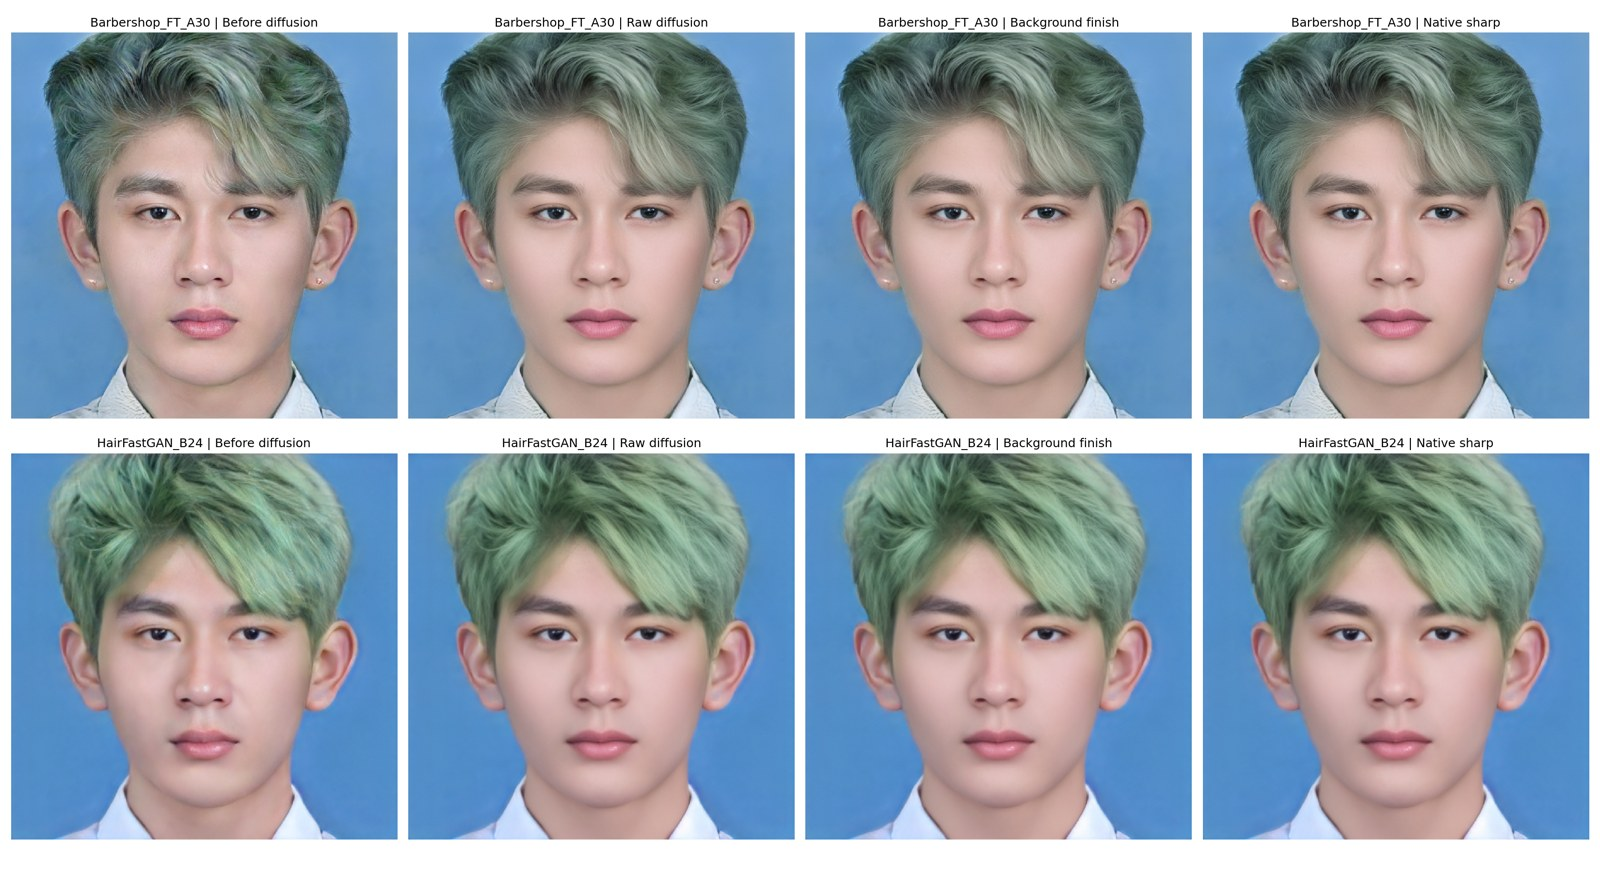
\includegraphics[width=0.95\textwidth]{images/diff_case1.jpg}
\caption{ชุดที่ 1}
\end{subfigure}

\vspace{0.4em}
\begin{subfigure}{\textwidth}
\centering
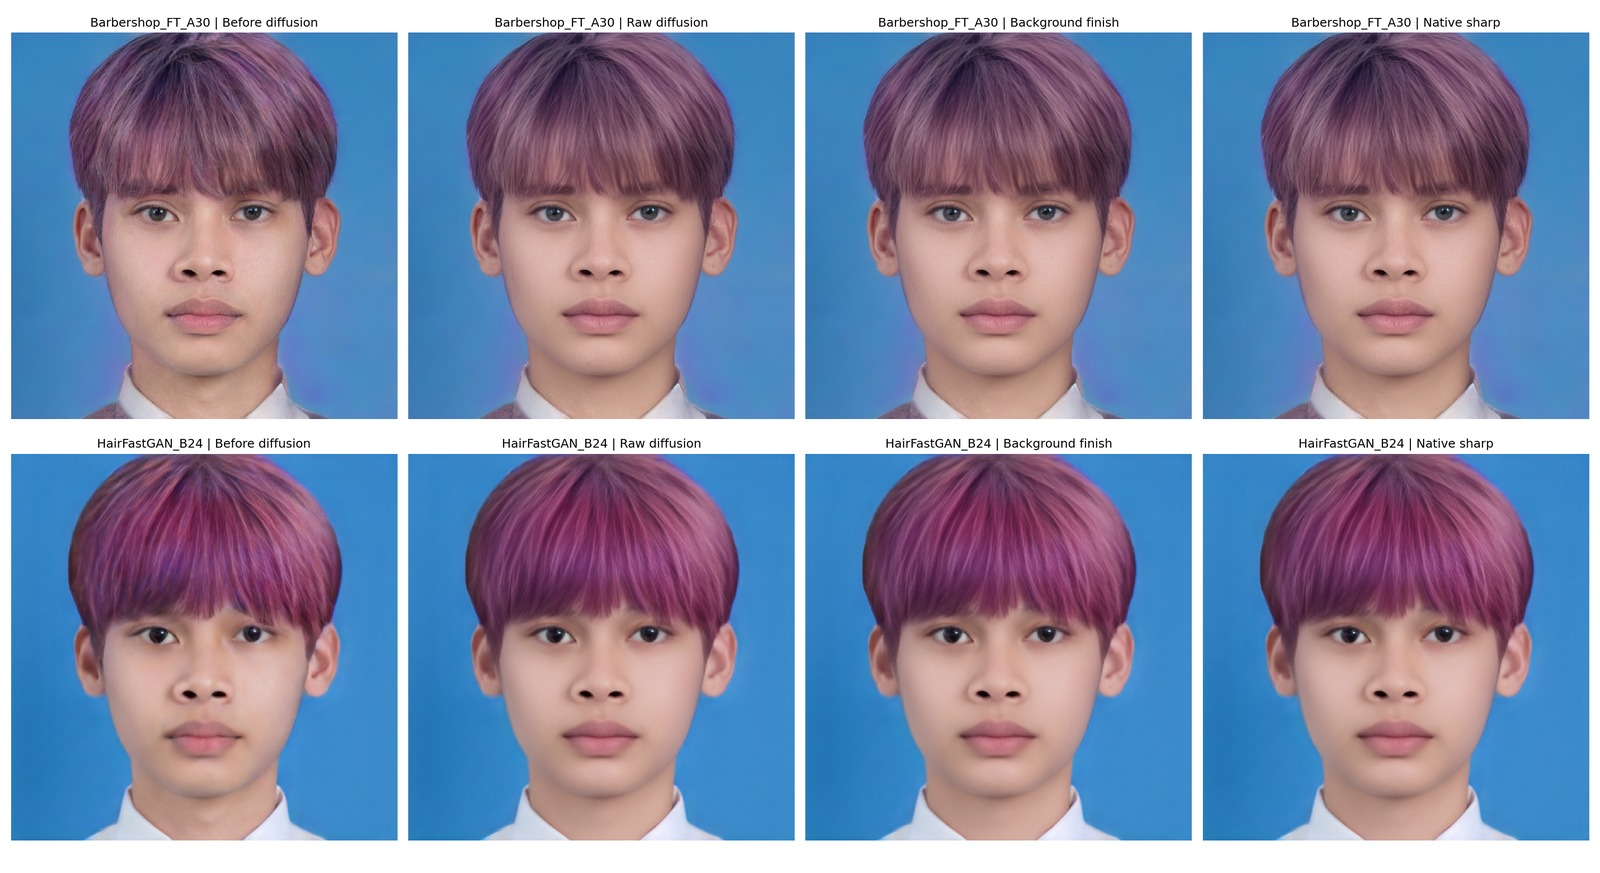
\includegraphics[width=0.95\textwidth]{images/diff_case2.jpg}
\caption{ชุดที่ 3}
\end{subfigure}
\caption{ตัวอย่างภาพหลังแต่ละขั้นของการขัดเกลา 2 ชุดจาก 8 ชุด (แถวบน BS-FT A30, แถวล่าง HFG B24)}
\label{fig:diff_cases}
\par\vspace{3pt}{\footnotesize\raggedright หมายเหตุ: BS-FT (Barbershop-FT) = Barbershop ที่ปรับจูนแล้ว (Fine-tuned), A30 = น้ำหนักของ Trial A Epoch 30, HFG = HairFastGAN, B24 = น้ำหนักของ Trial B Epoch 24\par}
\end{figure}

ตารางที่~\ref{tab:diff_result} แสดงผลของทุกชุด คอลัมน์ MUSIQ (Multi-scale Image Quality Transformer) และ ArcFace
แสดงค่าก่อน Diffusion และหลังขั้นสุดท้าย ArcFace ในตารางนี้คือความคล้ายของใบหน้าเทียบกับรูปต้นฉบับของผู้ใช้
คอลัมน์ IoU คือความทับกันของผมหลังขัดเกลาเทียบกับผมก่อนขัดเกลา
ส่วน MAE และ SSIM วัดเฉพาะพื้นที่นอกหน้ากากเทียบกับภาพก่อนขัดเกลา สองแถวล่างคือค่าเฉลี่ยของ 8 ชุด
ภาพที่~\ref{fig:diff_num} แสดง MUSIQ และ ArcFace ทีละขั้นเป็นกราฟเส้น แกนนอนคือขั้นตอน แกนตั้งคือค่าตัวชี้วัด
เส้นสีส้มคือ HFG เส้นสีน้ำเงินคือ BS-FT เส้นจางแต่ละเส้นคือหนึ่งชุดภาพ และเส้นเข้มคือค่าเฉลี่ย

\begin{table}[!htbp]
\centering
\caption{ผลของการขัดเกลาด้วย Diffusion ใน 8 ชุดภาพ}
\label{tab:diff_result}
\footnotesize
\begin{tabular}{|c|l|c|c|c|c|c|}
\hline
\textbf{ชุด} & \textbf{โมเดล} & \textbf{MUSIQ} $\uparrow$ & \textbf{ArcFace} $\uparrow$ & \textbf{IoU} $\uparrow$ & \textbf{MAE} $\downarrow$ & \textbf{SSIM} $\uparrow$ \\ \hline
1 & HFG & 64.00 $\rightarrow$ 62.62 & 0.900 $\rightarrow$ 0.779 & 0.968 & 0.0045 & 0.981 \\ \hline
1 & BS-FT & 77.79 $\rightarrow$ 77.99 & 0.769 $\rightarrow$ 0.622 & 0.977 & 0.0054 & 0.970 \\ \hline
2 & HFG & 67.96 $\rightarrow$ 67.07 & 0.754 $\rightarrow$ 0.599 & 0.990 & 0.0044 & 0.981 \\ \hline
2 & BS-FT & 77.49 $\rightarrow$ 77.48 & 0.733 $\rightarrow$ 0.548 & 0.993 & 0.0038 & 0.982 \\ \hline
3 & HFG & 68.06 $\rightarrow$ 67.84 & 0.805 $\rightarrow$ 0.774 & 0.986 & 0.0042 & 0.979 \\ \hline
3 & BS-FT & 76.17 $\rightarrow$ 76.01 & 0.726 $\rightarrow$ 0.655 & 0.989 & 0.0059 & 0.958 \\ \hline
4 & HFG & 57.74 $\rightarrow$ 54.32 & 0.832 $\rightarrow$ 0.772 & 0.992 & 0.0022 & 0.998 \\ \hline
4 & BS-FT & 71.36 $\rightarrow$ 71.37 & 0.726 $\rightarrow$ 0.658 & 0.984 & 0.0038 & 0.987 \\ \hline
5 & HFG & 59.68 $\rightarrow$ 58.42 & 0.892 $\rightarrow$ 0.829 & 0.975 & 0.0054 & 0.986 \\ \hline
5 & BS-FT & 76.26 $\rightarrow$ 75.86 & 0.769 $\rightarrow$ 0.711 & 0.984 & 0.0078 & 0.947 \\ \hline
6 & HFG & 65.67 $\rightarrow$ 65.24 & 0.821 $\rightarrow$ 0.735 & 0.992 & 0.0044 & 0.980 \\ \hline
6 & BS-FT & 75.20 $\rightarrow$ 77.06 & 0.804 $\rightarrow$ 0.680 & 0.984 & 0.0056 & 0.968 \\ \hline
7 & HFG & 69.35 $\rightarrow$ 65.06 & 0.835 $\rightarrow$ 0.751 & 0.978 & 0.0075 & 0.934 \\ \hline
7 & BS-FT & 77.00 $\rightarrow$ 76.14 & 0.793 $\rightarrow$ 0.678 & 0.976 & 0.0154 & 0.789 \\ \hline
8 & HFG & 56.33 $\rightarrow$ 53.52 & 0.622 $\rightarrow$ 0.497 & 0.983 & 0.0030 & 0.990 \\ \hline
8 & BS-FT & 69.95 $\rightarrow$ 68.85 & 0.500 $\rightarrow$ 0.439 & 0.984 & 0.0042 & 0.978 \\ \hline
\textbf{เฉลี่ย} & \textbf{HFG} & 63.60 $\rightarrow$ 61.76 & 0.808 $\rightarrow$ 0.717 & 0.983 & 0.0045 & 0.979 \\ \hline
\textbf{เฉลี่ย} & \textbf{BS-FT} & 75.15 $\rightarrow$ 75.09 & 0.728 $\rightarrow$ 0.624 & 0.984 & 0.0065 & 0.947 \\ \hline
\end{tabular}
\par\vspace{3pt}{\footnotesize\raggedright หมายเหตุ: MUSIQ = Multi-scale Image Quality Transformer (คะแนนคุณภาพภาพ), ArcFace = โมเดลจดจำใบหน้าที่ใช้วัดความเหมือนของใบหน้า, IoU = Intersection over Union (สัดส่วนพื้นที่ผมที่ทับกัน), MAE = Mean Absolute Error (ค่าความคลาดเคลื่อนสัมบูรณ์เฉลี่ย), SSIM = Structural Similarity Index (ดัชนีความคล้ายเชิงโครงสร้าง), HFG = HairFastGAN B24, BS-FT (Barbershop-FT) = Barbershop ที่ปรับจูนแล้ว (Fine-tuned) A30, $\rightarrow$ = จากก่อน Diffusion ไปหลังขั้นสุดท้าย\par}

\end{table}

\begin{figure}[!htbp]
\centering
\begin{subfigure}{0.49\textwidth}
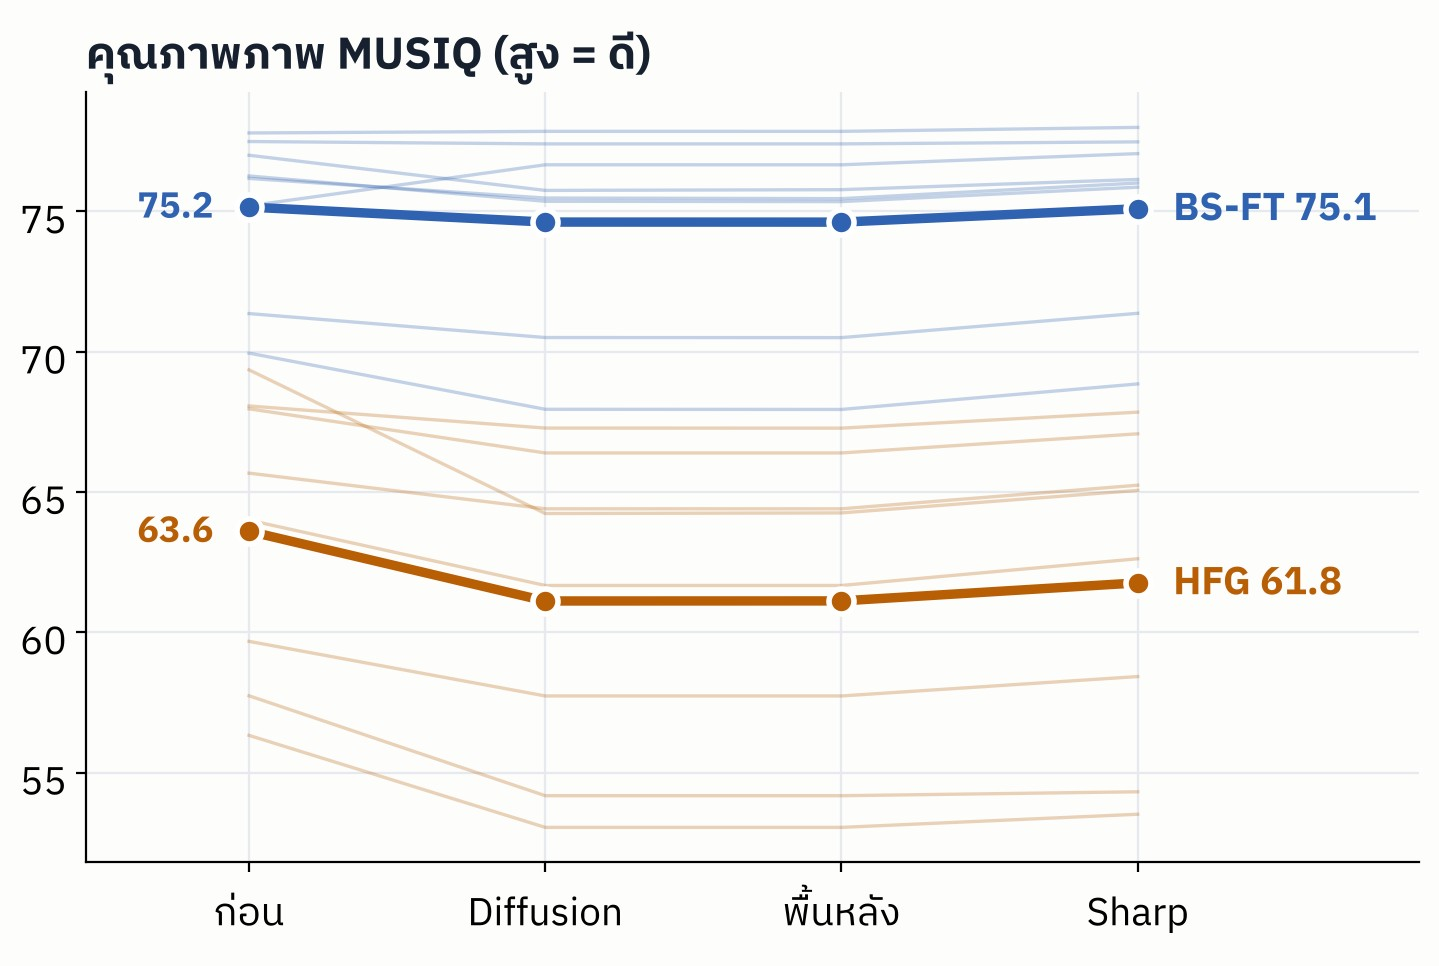
\includegraphics[width=\textwidth]{images/08_diff_musiq.jpg}
\caption{MUSIQ}
\end{subfigure}
\hfill
\begin{subfigure}{0.49\textwidth}
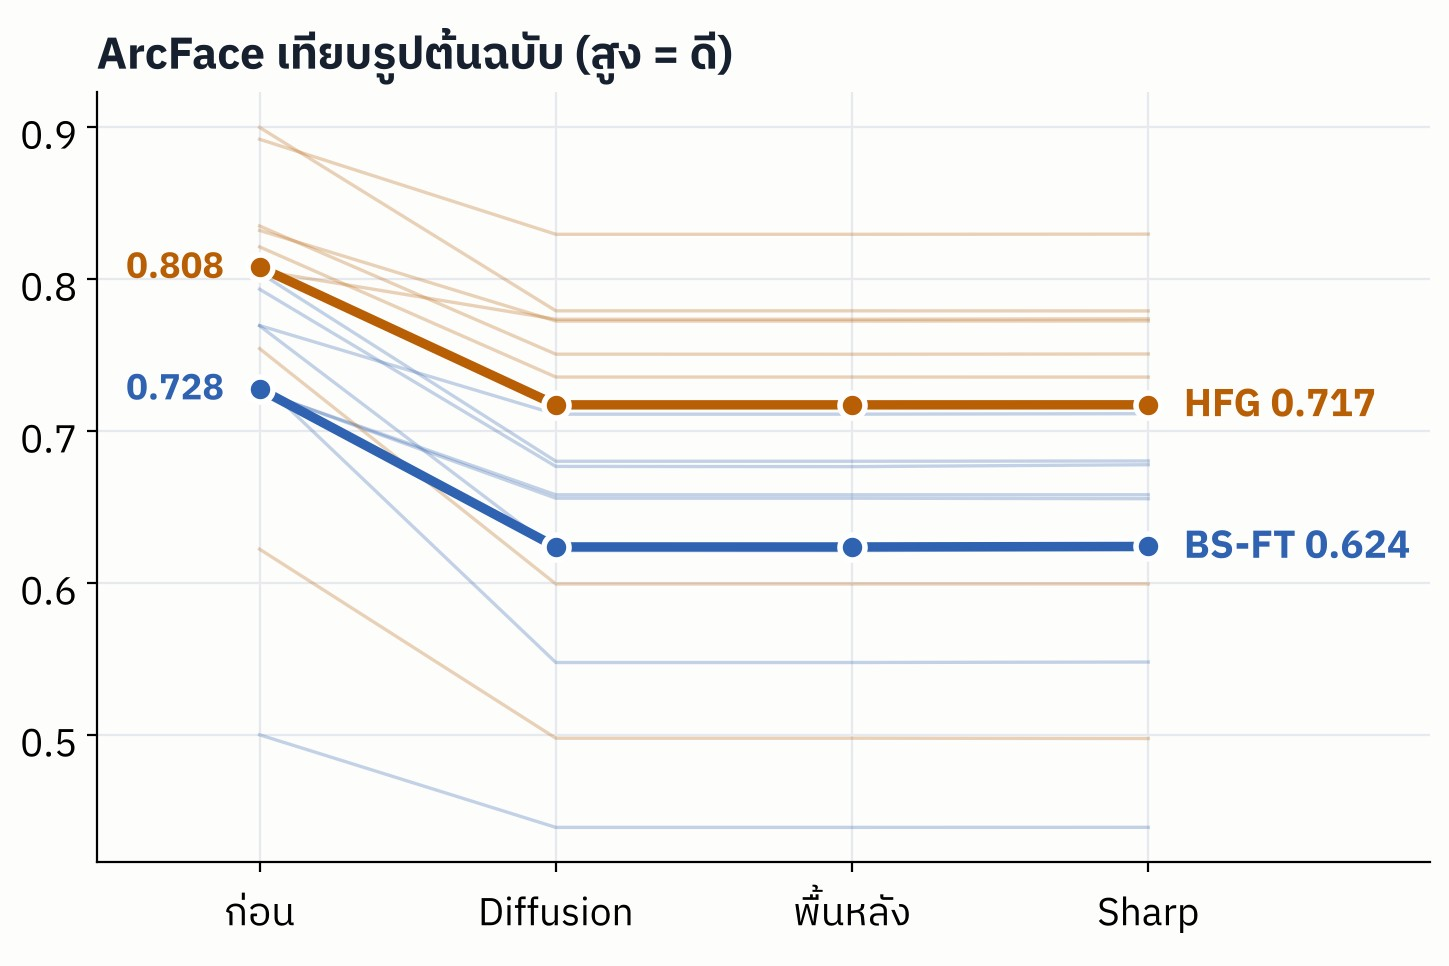
\includegraphics[width=\textwidth]{images/09_diff_arcface.jpg}
\caption{ArcFace}
\end{subfigure}
\caption{คุณภาพภาพและเอกลักษณ์ใบหน้าหลังแต่ละขั้นของการขัดเกลา (เส้นจาง = แต่ละชุดภาพ, เส้นเข้ม = ค่าเฉลี่ย 8 ชุด)}
\label{fig:diff_num}
\par\vspace{3pt}{\footnotesize\raggedright หมายเหตุ: MUSIQ = Multi-scale Image Quality Transformer (คะแนนคุณภาพภาพ), ArcFace = โมเดลจดจำใบหน้าที่ใช้วัดความเหมือนของใบหน้า, HFG = HairFastGAN, BS-FT (Barbershop-FT) = Barbershop ที่ปรับจูนแล้ว (Fine-tuned)\par}
\end{figure}

เมื่อเทียบกับเกณฑ์ในตารางที่~\ref{tab:diff_criteria} ได้ผลดังนี้
MUSIQ ของ HFG ลดลงทั้ง 8 ชุด เฉลี่ย $-1.84$ คะแนน (ลดน้อยที่สุด 0.22 และมากที่สุด 4.29)
ส่วนของ BS-FT แทบไม่เปลี่ยน เฉลี่ย $-0.06$ คะแนน (ตั้งแต่ $-1.10$ ถึง $+1.86$)
มีเพียงชุดที่ 6 ของ BS-FT ที่เพิ่มถึง +1 จึงผ่านเกณฑ์เพียง 1 จาก 16 กรณี
ArcFace ลดลงทุกกรณี HFG ลดเฉลี่ย 0.091 (0.032--0.155) และ BS-FT ลดเฉลี่ย 0.104 (0.058--0.185)
จึงไม่ผ่านเกณฑ์ที่ให้ลดได้ไม่เกิน 0.02 ในทุกกรณี
ด้านทรงผม IoU เทียบกับภาพก่อน Diffusion อยู่ระหว่าง 0.968--0.993 ผ่านเกณฑ์ 0.97 ใน 15 จาก 16 กรณี
มีเพียงชุดที่ 1 ของ HFG ที่ได้ 0.968 ซึ่งต่ำกว่าเกณฑ์เล็กน้อย
ด้านพื้นที่นอกหน้ากาก HFG ผ่านทั้ง MAE และ SSIM ใน 5 จาก 8 ชุด (MAE เฉลี่ย 0.0045, SSIM เฉลี่ย 0.979)
ส่วน BS-FT ผ่านเพียง 2 จาก 8 ชุด (MAE เฉลี่ย 0.0065, SSIM เฉลี่ย 0.947)
โดยชุดที่ 7 ของ BS-FT เปลี่ยนมากที่สุด (MAE 0.0154, SSIM 0.789) ซึ่งต้องตรวจภาพเป็นรายกรณีต่อไป
พื้นที่นี้ไม่ได้ถูก Diffusion วาดใหม่ ความต่างที่ไม่เป็นศูนย์ส่วนใหญ่มาจากการที่ทั้งภาพต้องผ่านการบีบอัดและคืนสภาพของ VAE
(หัวข้อที่~\ref{sec:stablediffusion}) และบางส่วนมาจากขั้นเก็บพื้นหลังที่ตั้งใจแก้พื้นหลังอยู่แล้ว
ด้านสี ความคลาดเคลื่อนในช่อง $a$ และ $b$ ของ BS-FT ลดลงใน 5 จาก 8 ชุด (เฉลี่ยจาก 2.52 เป็น 2.41)
แต่ของ HFG เพิ่มขึ้นทั้ง 8 ชุด (เฉลี่ยจาก 2.62 เป็น 3.09) แปลว่า Diffusion ทำให้สีผมของ HFG เพี้ยนจากเป้าหมายเล็กน้อย
กราฟยังบอกด้วยว่าการเปลี่ยนแปลงเกือบทั้งหมดเกิดในขั้น Diffusion
ขั้นเก็บพื้นหลังและ Native Sharp แทบไม่กระทบ ArcFace และ Native Sharp ช่วยดึง MUSIQ กลับขึ้นมาเล็กน้อยในทั้งสองโมเดล
ส่วนเวลาที่เพิ่มขึ้นจากการขัดเกลาทั้งหมดคือ 2.97--3.28 วินาทีสำหรับ HFG (เฉลี่ย 3.15)
และ 3.05--4.77 วินาทีสำหรับ BS-FT (เฉลี่ย 3.73)

ผู้วิจัยตีความว่าตัวเลขชุดนี้บอกได้เพียงครึ่งเดียว
ArcFace ที่ลดลงในทุกกรณีเป็นสัญญาณจริงว่าใบหน้าเปลี่ยน ซึ่งผู้วิจัยต้องยอมรับ
แต่ ArcFace วัดความคล้ายของใบหน้า ไม่ได้วัดคุณภาพของเส้นผม ส่วน MUSIQ ประเมินคุณภาพภาพโดยรวมโดยไม่ใช้ภาพอ้างอิง
คะแนนทั้งสองจึงควรพิจารณาร่วมกับคะแนนจากผู้ใช้ และจากกรณีศึกษานี้ยังระบุไม่ได้ว่าทำไมตัวเลขกับความเห็นของผู้ใช้จึงไปคนละทาง
การตัดสินว่าภาพดีขึ้นจริงหรือไม่จึงต้องให้ผู้ใช้เป็นผู้บอก ดังจะเห็นในหัวข้อที่~\ref{sec:subjective}

% -----------------------------------------------------------
\section{ผลการประเมินโดยผู้ใช้}
\label{sec:subjective}
% -----------------------------------------------------------

ผู้ใช้ 41 คนประเมินภาพจาก 4 ระบบโดยไม่รู้ชื่อโมเดล รวม 164 คำตอบ
ภาพที่~\ref{fig:result_examples} เป็นตัวอย่างภาพที่ผู้ใช้เห็น 2 ชุด
มุมซ้ายบนของแต่ละชุดคือภาพนำเข้า (ใบหน้า ทรงผม และสีผม) และแถวล่างคือผลของ 4 ระบบตามชื่อที่อยู่ใต้ภาพ
ถ้าดูคู่ภาพก่อนและหลัง Diffusion จะเห็นว่าผมที่ผ่าน Diffusion มีเส้นชัดขึ้น
และถ้าเทียบระหว่างโมเดล HFG ยังคงหน้าตาของเจ้าของภาพได้ใกล้กว่า BS-FT

\begin{figure}[!htbp]
\centering
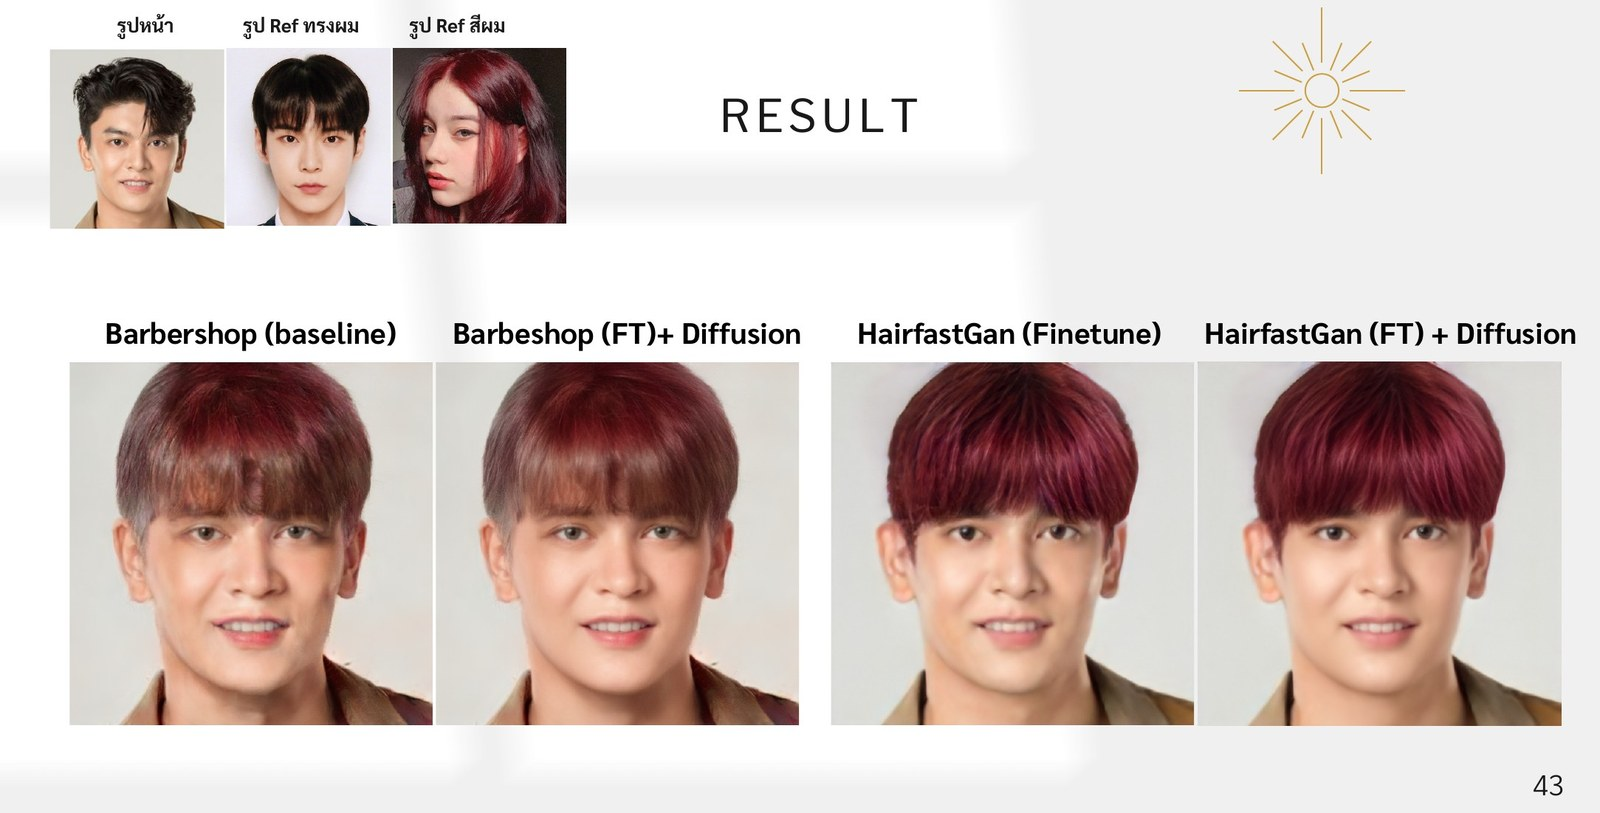
\includegraphics[width=\textwidth]{images/fig_result_1.jpg}

\vspace{0.3em}
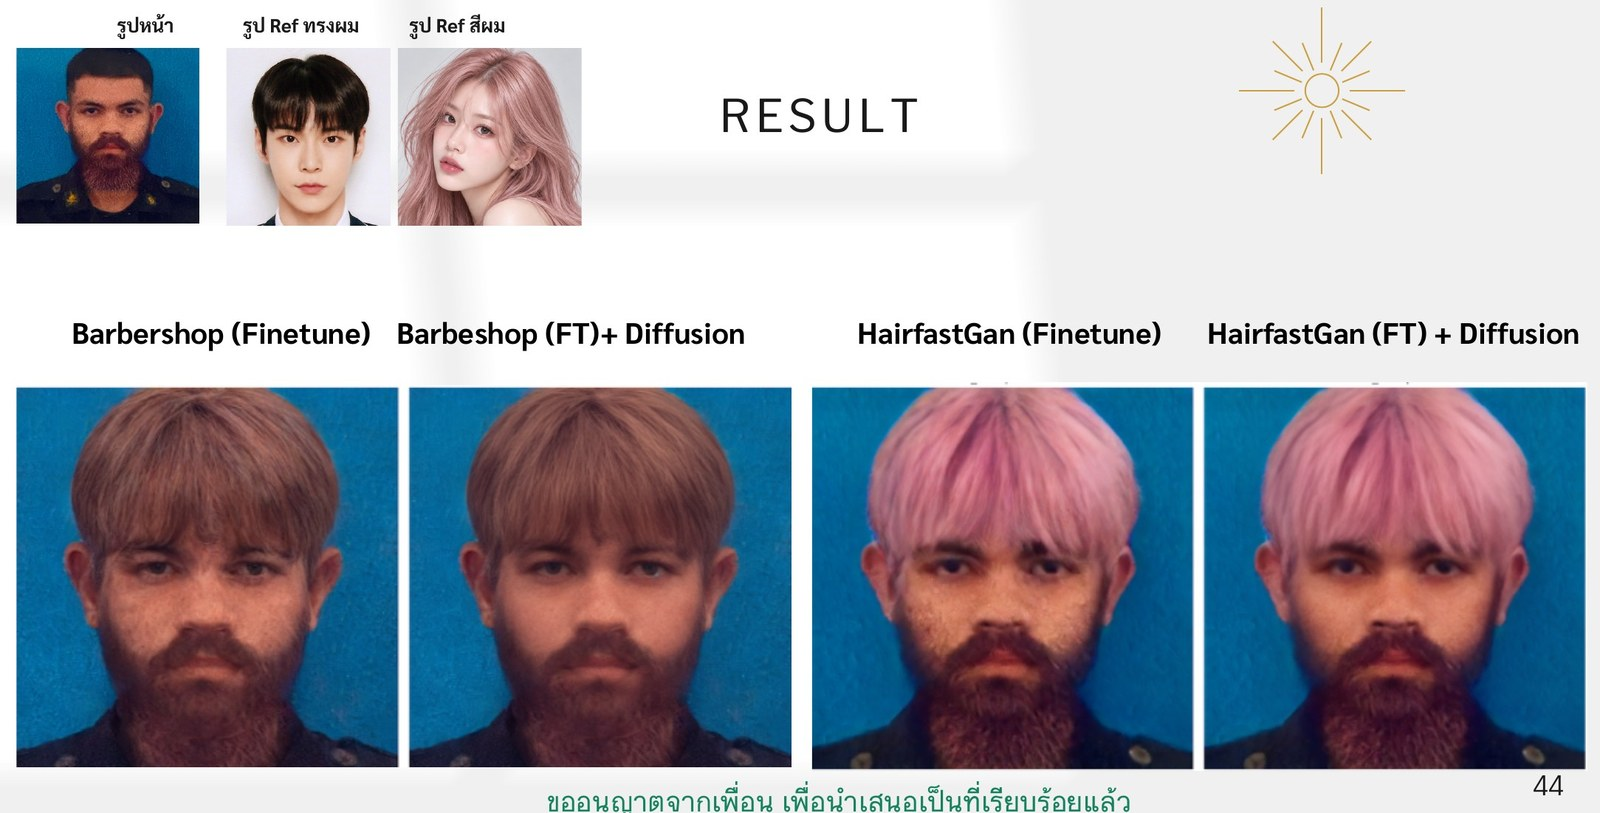
\includegraphics[width=\textwidth]{images/fig_result_2.jpg}
\caption{ตัวอย่างผลลัพธ์ของ 4 ระบบจากภาพนำเข้าชุดเดียวกัน}
\label{fig:result_examples}
\end{figure}

ภาพที่~\ref{fig:survey_form} คือหน้าแบบประเมินจริง ด้านซ้ายมีภาพใบหน้าของผู้ใช้ ภาพทรงผม ภาพสีผม
และภาพผลลัพธ์ทีละภาพ ด้านขวาคือคำถาม 6 ข้อตามตารางที่~\ref{tab:survey_q}
หน้านี้ไม่มีชื่อโมเดลอยู่เลย และลำดับภาพถูกสุ่มใหม่สำหรับทุกคน
ผู้ใช้จึงไม่มีทางรู้ว่ากำลังให้คะแนนระบบใด

\begin{figure}[!htbp]
\centering
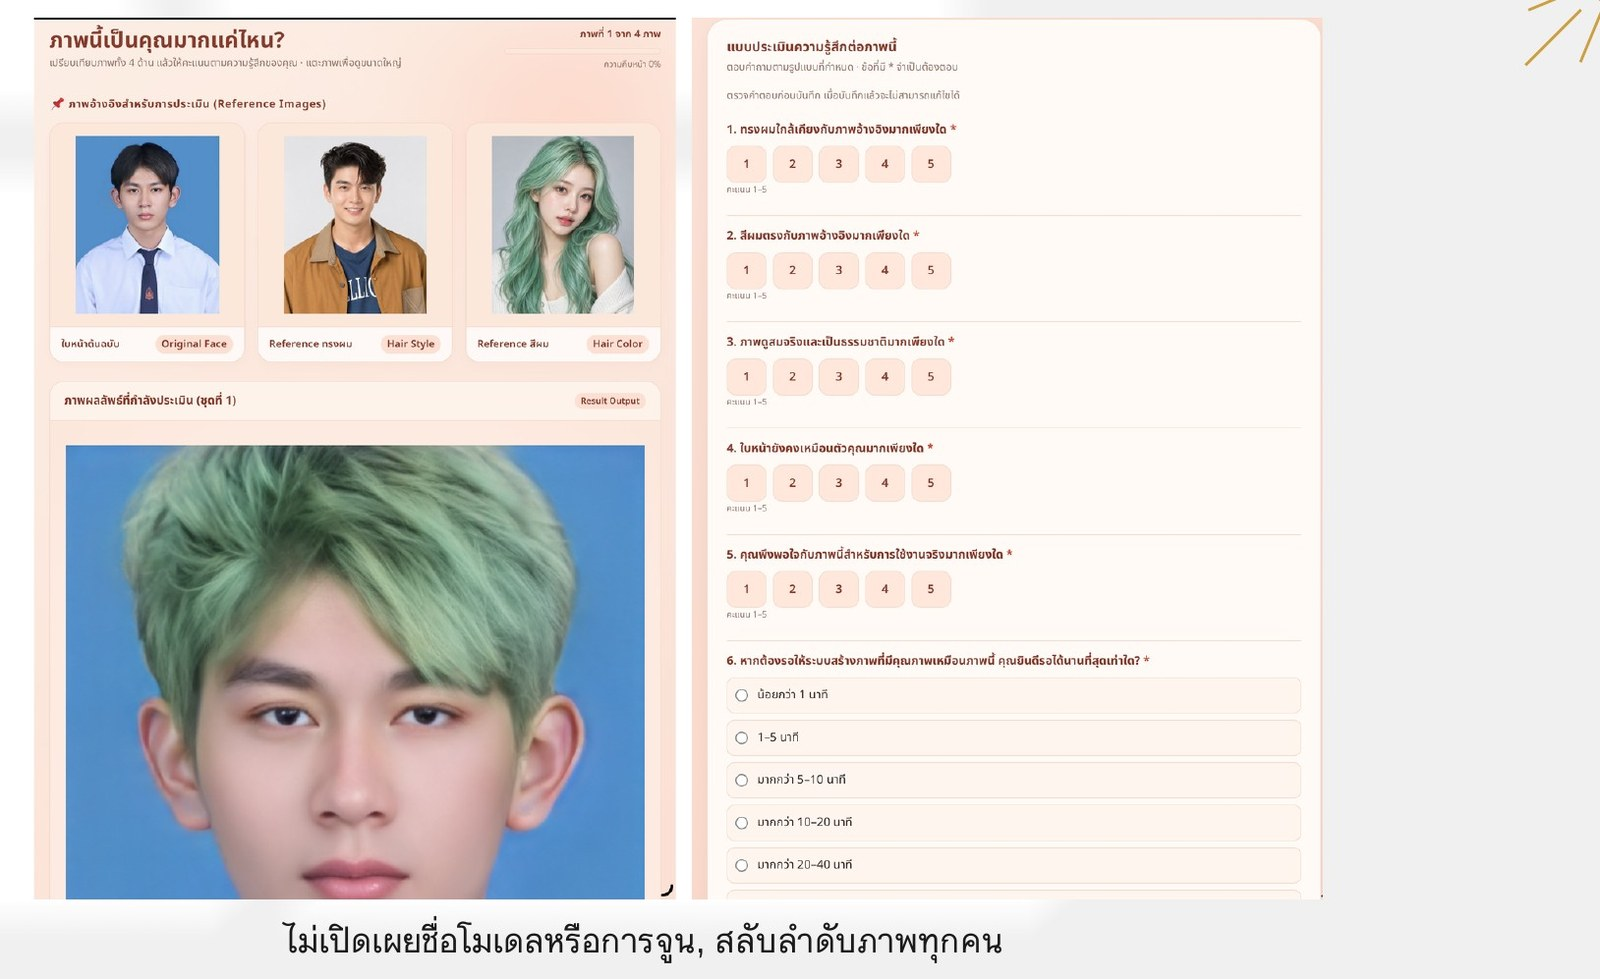
\includegraphics[width=0.75\textwidth]{images/fig_survey_form.jpg}
\caption{หน้าแบบประเมินที่ไม่เปิดเผยชื่อโมเดลและสลับลำดับภาพทุกคน}
\label{fig:survey_form}
\end{figure}

ตารางที่~\ref{tab:survey_mean} คือคะแนนเฉลี่ย (1--5) แต่ละแถวคือคำถามหนึ่งข้อ แต่ละคอลัมน์คือหนึ่งระบบ
ตัวหนาคือคะแนนสูงสุดของแถว และแถวสุดท้ายคือเวลาต่อภาพ
สิ่งแรกที่สังเกตได้คือไม่มีระบบใดชนะทุกข้อ
BS-FT + Diff ได้คะแนนทรงผมและความสมจริงสูงสุด HFG B24 + Diff ได้คะแนนสีผมและความพึงพอใจสูงสุด
ส่วน HFG B24 ที่ไม่ผ่าน Diffusion ได้คะแนนความเหมือนของใบหน้าสูงสุด
และถ้าดูแถวใบหน้าจะเห็นว่าคะแนนลดลงทุกครั้งที่ผ่าน Diffusion ทั้งสองโมเดล
ซึ่งตรงกับค่า ArcFace ที่ลดลงในหัวข้อก่อน

\begin{table}[!htbp]
\centering
\caption{คะแนนเฉลี่ยจากผู้ใช้ 41 คน (คะแนน 1--5)}
\label{tab:survey_mean}
\small
\begin{tabular}{|l|c|c|c|c|}
\hline
\textbf{คำถาม} & \textbf{HFG B24} & \textbf{HFG B24 + Diff} & \textbf{BS-FT A30} & \textbf{BS-FT A30 + Diff} \\ \hline
ทรงผมตรงภาพอ้างอิง & 3.68 & 3.88 & 3.80 & \textbf{4.10} \\ \hline
สีผมตรงภาพอ้างอิง & 4.05 & \textbf{4.22} & 3.90 & 4.17 \\ \hline
สมจริง เป็นธรรมชาติ & 3.37 & 3.46 & 3.24 & \textbf{3.83} \\ \hline
ใบหน้ายังเหมือนตัวเอง & \textbf{4.17} & 3.95 & 3.54 & 3.22 \\ \hline
พึงพอใจใช้งานจริง & 3.66 & \textbf{3.90} & 3.63 & 3.83 \\ \hline
เวลาต่อภาพ & $\approx$ 10 วินาที & $\approx$ 13 วินาที & $\approx$ 11 นาที & $\approx$ 11 นาที \\ \hline
\end{tabular}
\par\vspace{3pt}{\footnotesize\raggedright หมายเหตุ: HFG = HairFastGAN, B24 = น้ำหนักของ Trial B Epoch 24, Diff = ขั้นขัดเกลาด้วย Diffusion, BS-FT (Barbershop-FT) = Barbershop ที่ปรับจูนแล้ว (Fine-tuned), A30 = น้ำหนักของ Trial A Epoch 30\par}

\end{table}

\subsection{ผลของ Diffusion ในสายตาผู้ใช้}

เพื่อดูผลของ Diffusion อย่างเดียว ผู้วิจัยเทียบคะแนนที่คนเดียวกันให้ภาพก่อนและหลัง Diffusion
ภาพที่~\ref{fig:survey_diff} แยกเป็น (a) HFG B24 และ (b) BS-FT A30
แต่ละแถวคือคำถามหนึ่งข้อ จุดสีเทาคือคะแนนก่อน Diffusion จุดสีคือคะแนนหลัง Diffusion
ตัวเลขด้านขวาคือผลต่าง (สีเขียว = ดีขึ้น สีแดง = แย่ลง) และเครื่องหมาย * หมายถึงช่วงความเชื่อมั่น 95\% ไม่ครอบคลุมเลข 0
ตารางที่~\ref{tab:survey_pair} ให้ตัวเลขชุดเดียวกันพร้อมช่วงความเชื่อมั่น
คอลัมน์ที่สองและสามคือผลของ Diffusion ในแต่ละโมเดล
ส่วนคอลัมน์สุดท้ายเทียบ HFG + Diff กับ BS-FT + Diff โดยตรง ซึ่งใช้ตอนเลือกโมเดลไปใช้บนเว็บ

\begin{figure}[!htbp]
\centering
\begin{subfigure}{0.49\textwidth}
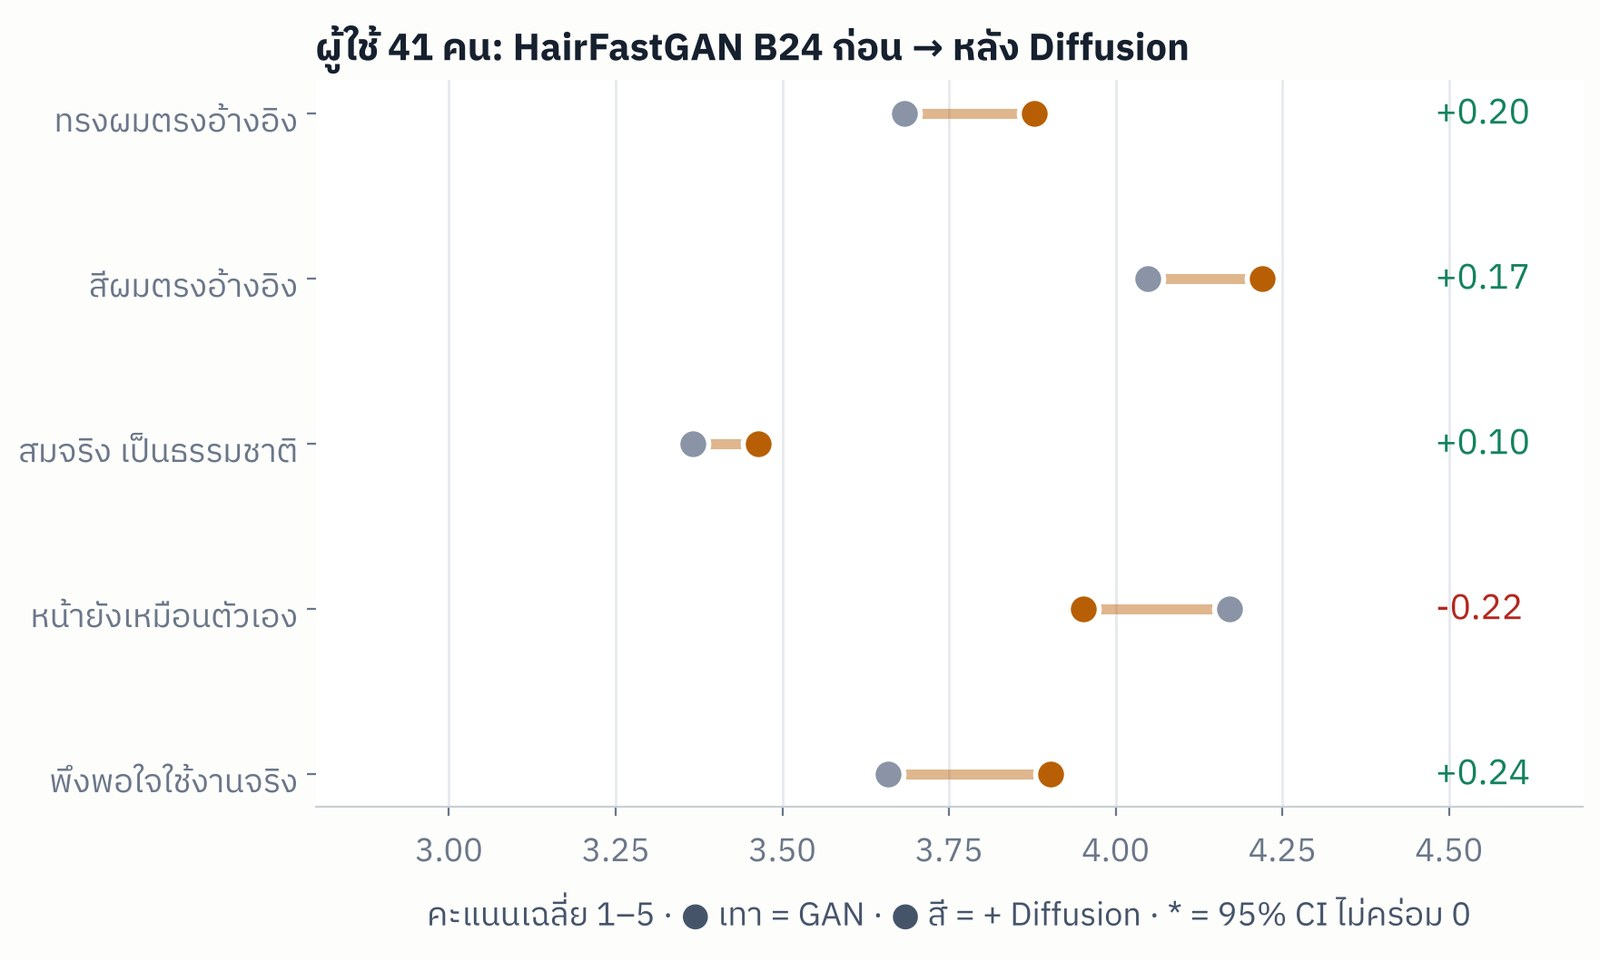
\includegraphics[width=\textwidth]{images/10_survey_hfg.jpg}
\caption{HairFastGAN B24}
\end{subfigure}
\hfill
\begin{subfigure}{0.49\textwidth}
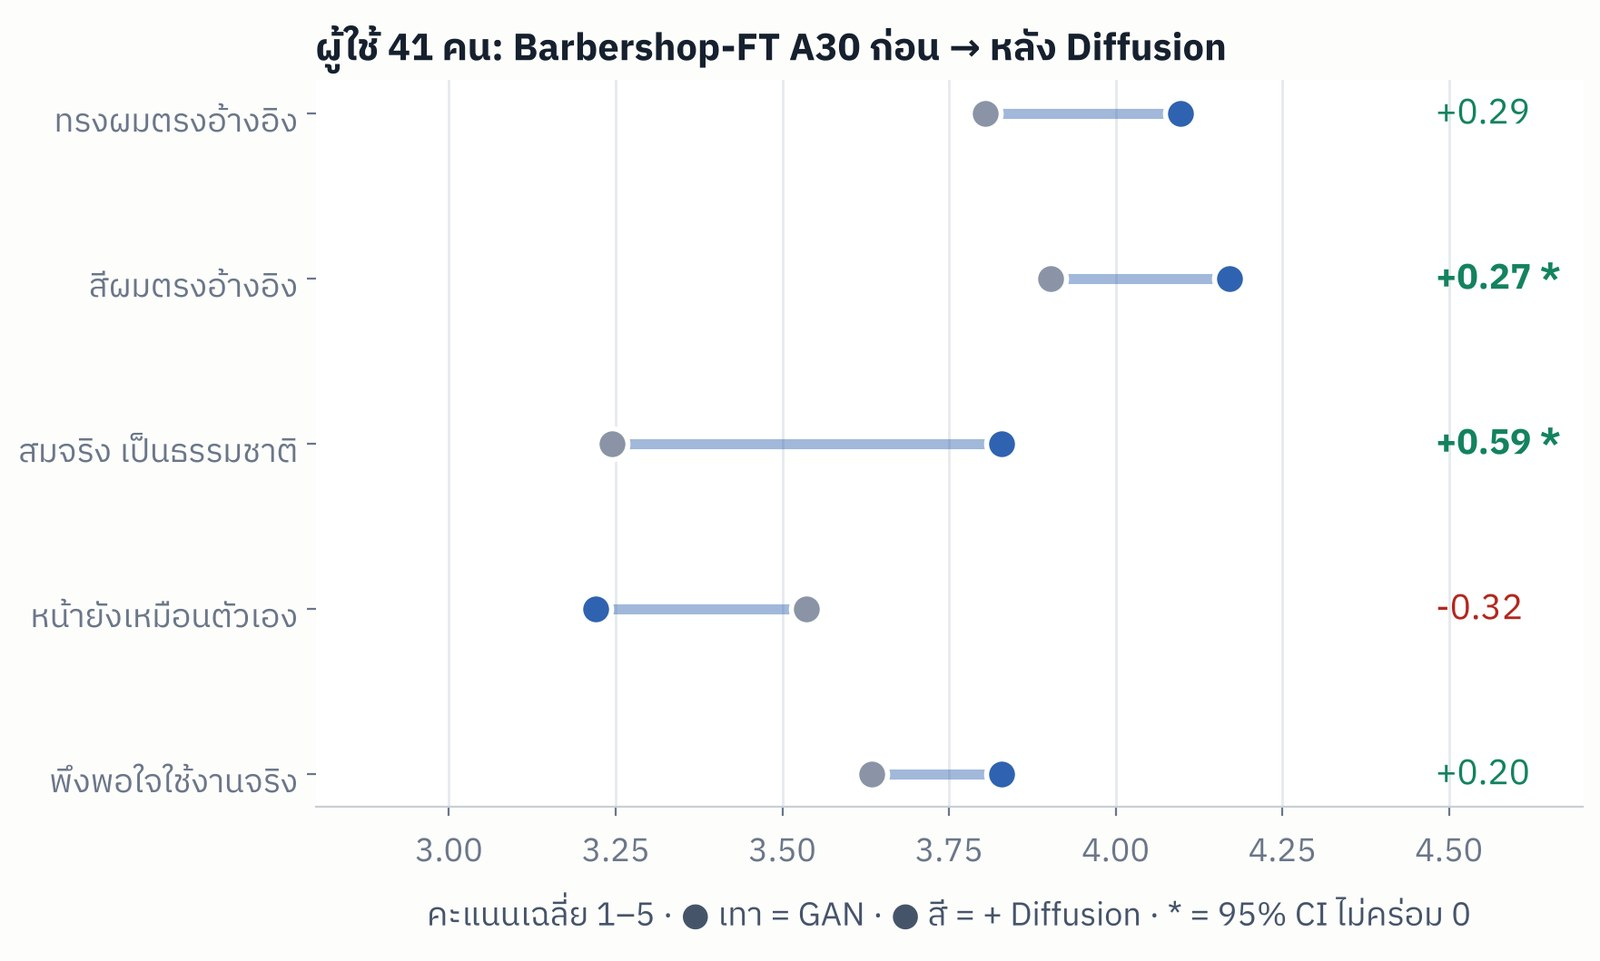
\includegraphics[width=\textwidth]{images/11_survey_bs.jpg}
\caption{Barbershop-FT A30}
\end{subfigure}
\caption{คะแนนผู้ใช้ก่อน (จุดเทา) และหลัง Diffusion (จุดสี)
เครื่องหมาย * คือช่วงความเชื่อมั่น 95\% ไม่คร่อมศูนย์}
\label{fig:survey_diff}
\par\vspace{3pt}{\footnotesize\raggedright หมายเหตุ: B24 = น้ำหนักของ Trial B Epoch 24, BS-FT (Barbershop-FT) = Barbershop ที่ปรับจูนแล้ว (Fine-tuned), A30 = น้ำหนักของ Trial A Epoch 30, HFG = HairFastGAN, GAN = Generative Adversarial Network, CI = Confidence Interval (ช่วงความเชื่อมั่น)\par}
\end{figure}

\begin{table}[!htbp]
\centering
\caption{ผลต่างคะแนนแบบจับคู่รายคน (95\% CI จากบูตสแตรป)}
\label{tab:survey_pair}
\footnotesize
\begin{tabular}{|l|c|c|c|}
\hline
\textbf{คำถาม} & \textbf{HFG + Diff $-$ HFG} & \textbf{BS-FT + Diff $-$ BS-FT} & \textbf{HFG + Diff $-$ BS-FT + Diff} \\ \hline
ทรงผม & $+0.20$ ($-0.02$, $+0.41$) & $+0.29$ ($-0.02$, $+0.63$) & $-0.22$ ($-0.54$, $+0.10$) \\ \hline
สีผม & $+0.17$ ($-0.05$, $+0.37$) & $+0.27$ ($+0.02$, $+0.51$) & $+0.05$ ($-0.32$, $+0.44$) \\ \hline
สมจริง & $+0.10$ ($-0.17$, $+0.37$) & $+0.59$ ($+0.27$, $+0.93$) & $-0.37$ ($-0.63$, $-0.12$) \\ \hline
ใบหน้าเหมือนตัวเอง & $-0.22$ ($-0.46$, $+0.02$) & $-0.32$ ($-0.66$, $0.00$) & $+0.73$ ($+0.37$, $+1.10$) \\ \hline
พึงพอใจใช้งานจริง & $+0.24$ ($0.00$, $+0.49$) & $+0.20$ ($-0.10$, $+0.49$) & $+0.07$ ($-0.24$, $+0.37$) \\ \hline
\end{tabular}
\par\vspace{3pt}{\footnotesize\raggedright หมายเหตุ: CI = Confidence Interval (ช่วงความเชื่อมั่น), HFG = HairFastGAN, Diff = ขั้นขัดเกลาด้วย Diffusion, BS-FT (Barbershop-FT) = Barbershop ที่ปรับจูนแล้ว (Fine-tuned)\par}

\end{table}

ผลที่ชัดที่สุดคือความสมจริงของ BS-FT ซึ่งเพิ่มขึ้น $+0.59$ (95\% CI $+0.27$ ถึง $+0.93$)
มีผู้ใช้ 20 คนให้คะแนนสูงขึ้น และมีเพียง 4 คนที่ให้คะแนนต่ำลง
ขณะที่ความสมจริงของ HFG เพิ่มเพียง $+0.10$ ผู้วิจัยคิดว่าเป็นเพราะภาพของ BS-FT มีรายละเอียดผมเป็นพื้นฐานอยู่แล้ว
Diffusion แบบแรงต่ำจึงต่อยอดได้ดี ส่วนผมของ HFG เรียบกว่า จึงมีรายละเอียดตั้งต้นให้ Diffusion ใช้น้อยกว่า
สำหรับทรงและสีผม คะแนนเฉลี่ยเพิ่มขึ้นเล็กน้อยในกลุ่มตัวอย่างที่ประเมิน
โดยมีผลต่าง $+0.17$ ถึง $+0.29$
อย่างไรก็ตาม การที่ไม่พบว่าคะแนนลดลงไม่ได้พิสูจน์ว่า Diffusion ไม่ทำให้ทรงและสีผมแย่ลงเลย
ส่วนสีผมของ BS-FT เพิ่มขึ้นอย่างชัดเจน ($+0.27$; $+0.02$ ถึง $+0.51$)
ด้านที่เสียคือความเหมือนของใบหน้า (HFG $-0.22$ และ BS-FT $-0.32$) ซึ่งไปทางเดียวกับ ArcFace
แต่เมื่อรวมทุกด้านแล้ว ผู้ใช้ยังพอใจมากขึ้น HFG $+0.24$ (95\% CI 0.00 ถึง $+0.49$) และ BS-FT $+0.20$
ผลนี้สะท้อนแนวโน้มของคะแนนเฉลี่ย แต่ยังไม่ยืนยันว่าผู้ใช้ส่วนใหญ่ยอมแลกความเหมือนของใบหน้ากับรายละเอียดของผม
โดยเฉพาะผลต่างความพึงพอใจของ BS-FT ที่ช่วงความเชื่อมั่นครอบคลุมเลข 0 และของ HFG ที่ขอบล่างปัดเศษแล้วเป็น 0

\subsection{เวลาที่ผู้ใช้ยอมรอ}

คำถามข้อ 6 ตอบเรื่องที่ตัวชี้วัดใดก็ตอบไม่ได้ คือผู้ใช้ยอมรอได้นานเท่าใด
ภาพที่~\ref{fig:survey_wait} แกนตั้งคือช่วงเวลา แกนนอนคือร้อยละของคำตอบ (41 คน $\times$ 4 ภาพ)
และแท่งสีเข้มคือช่วงที่ไม่เกิน 5 นาที
ร้อยละ 84 ของคำตอบยอมรอได้ไม่เกิน 5 นาที คือ 137 จาก 164 คำตอบ (น้อยกว่า 1 นาที 38 คำตอบ และ 1--5 นาที 99 คำตอบ)
ร้อยละ 12 ยอมรอ 5--10 นาที (20 คำตอบ) และมีเพียงร้อยละ 4 ที่ยอมรอเกิน 10 นาที (7 คำตอบ)
ตัวเลขนี้ทำให้เห็นภาพชัดขึ้นมาก HFG + Diff ใช้เวลาประมาณ 13 วินาที ซึ่งสั้นกว่าขอบบนของช่วงเวลาที่สั้นที่สุดในแบบสอบถาม
แต่ยังยืนยันไม่ได้ว่าทุกคนยอมรับเวลา 13 วินาที
ขณะที่ BS-FT + Diff ใช้ประมาณ 11 นาที ซึ่งนานเกินกว่าที่ร้อยละ 96 ของคำตอบยอมรอ
ไม่ว่าภาพจะสวยเพียงใด ถ้าผู้ใช้ไม่ยอมรอ ภาพนั้นก็ไม่ถูกใช้

\begin{figure}[!htbp]
\centering
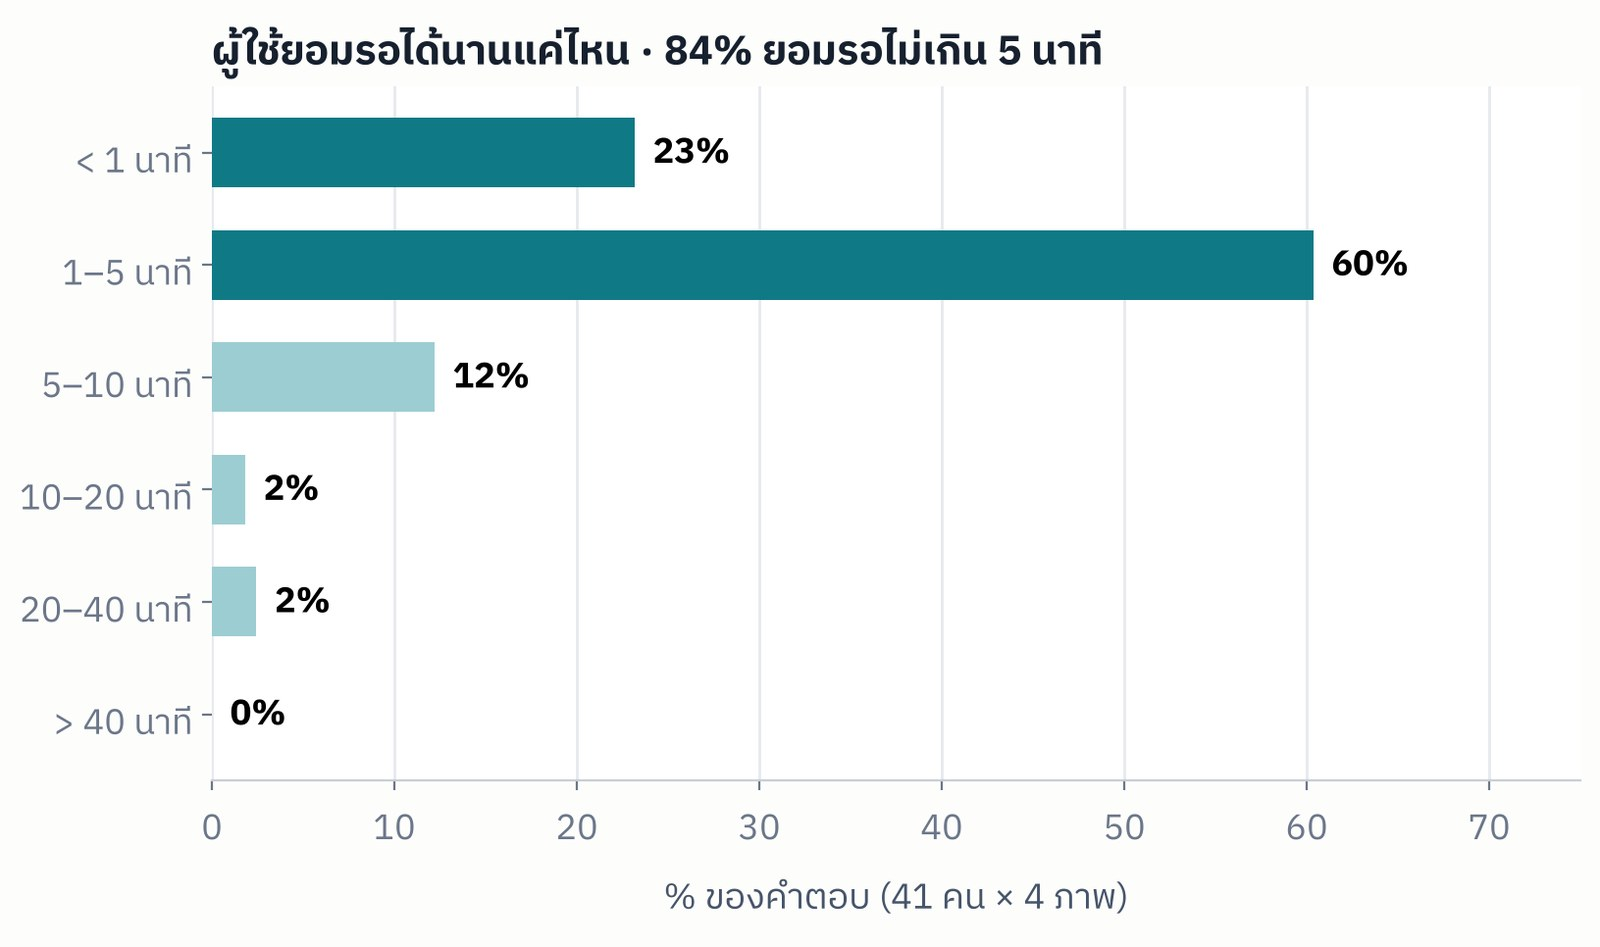
\includegraphics[width=0.75\textwidth]{images/12_survey_wait.jpg}
\caption{เวลาที่ผู้ใช้ยอมรอเพื่อให้ได้ภาพคุณภาพเท่าภาพที่เห็น (41 คน $\times$ 4 ภาพ)}
\label{fig:survey_wait}
\end{figure}

\subsection{สรุปผลของ Diffusion จากตัวเลขและผู้ใช้}

ตารางที่~\ref{tab:diff_decision} วางผลจากตัวเลขกับผลจากผู้ใช้ไว้คู่กันทีละด้าน
คอลัมน์ที่สองคือผลจากตัวเลข คอลัมน์ที่สามคือผลจากผู้ใช้ และคอลัมน์สุดท้ายคือข้อสรุป
ในกรณีศึกษาเชิงตัวเลข MUSIQ ลดลง แต่คะแนนความสมจริงจากผู้ใช้เพิ่มขึ้น โดยผลของ BS-FT ชัดกว่า HFG
MUSIQ ไม่ใช้ภาพอ้างอิง คะแนนที่ลดลงจึงไม่ได้เกิดจากการเทียบรายละเอียดใหม่กับภาพเดิมโดยตรง
และภาพในกรณีศึกษาเชิงตัวเลขกับภาพในแบบสอบถามเป็นคนละชุดกัน จึงยังระบุสาเหตุที่ผลไม่สอดคล้องกันไม่ได้
คะแนนเฉลี่ยของทรงและสีผมเพิ่มขึ้นเล็กน้อย แต่ยังไม่ได้ทดสอบทางสถิติโดยตรงว่าไม่แย่ลง
คะแนนเฉลี่ยความเหมือนของใบหน้าลดลง โดยช่วงความเชื่อมั่นยังแตะหรือครอบคลุมเลข 0
ส่วนความพึงพอใจเพิ่มขึ้นในค่าเฉลี่ย แต่ยังไม่ชัดเจนสำหรับทั้งสองโมเดล
สรุปได้ว่าผลจากผู้ใช้สนับสนุนว่า Diffusion ช่วยให้ภาพของ BS-FT สมจริงขึ้น
ขณะที่ผลต่อ HFG และการรักษาใบหน้ายังต้องประเมินเพิ่ม โดยมีเวลาประมวลผลเพิ่มเฉลี่ย 3.15 วินาทีสำหรับ HFG ในสภาพแวดล้อมที่ทดสอบ

\begin{table}[!htbp]
\centering
\caption{การตัดสินผลของ Diffusion จากตัวชี้วัดเชิงตัวเลขร่วมกับผู้ใช้}
\label{tab:diff_decision}
\small
\begin{tabular}{|l|L{3.4cm}|L{4.6cm}|L{2.2cm}|}
\hline
\textbf{ด้าน} & \textbf{ตัวชี้วัดเชิงตัวเลข} & \textbf{ผู้ใช้ (41 คน)} & \textbf{สรุป} \\ \hline
ความสมจริง & MUSIQ เปลี่ยน $-4.3$ ถึง $+1.9$ ถึงเกณฑ์ +1 เพียง 1 จาก 16 กรณี & BS-FT $+0.59$, HFG $+0.10$ & ผู้ใช้สนับสนุน BS-FT \\ \hline
ทรงและสีผม & IoU 0.968--0.993 ผ่านเกณฑ์ 0.97 ใน 15 จาก 16 กรณี & ดีขึ้นเล็กน้อย $+0.17$ ถึง $+0.29$ & ส่วนใหญ่ไม่เสีย \\ \hline
ใบหน้าเหมือนเดิม & ArcFace ลด 0.03--0.19 ทุกกรณี & ลดลง $-0.22$ ถึง $-0.32$ & ต้องปรับปรุง \\ \hline
ความพึงพอใจ & -- & ดีขึ้น $+0.20$ ถึง $+0.24$ & ช่วยเล็กน้อย \\ \hline
เวลา & เพิ่ม 3.0--4.8 วินาทีต่อภาพ & ส่วนใหญ่ยอมรอไม่เกิน 5 นาที & รับได้ \\ \hline
\end{tabular}
\par\vspace{3pt}{\footnotesize\raggedright หมายเหตุ: MUSIQ = Multi-scale Image Quality Transformer (คะแนนคุณภาพภาพ), BS-FT (Barbershop-FT) = Barbershop ที่ปรับจูนแล้ว (Fine-tuned), HFG = HairFastGAN, IoU = Intersection over Union (สัดส่วนพื้นที่ผมที่ทับกัน), ArcFace = โมเดลจดจำใบหน้าที่ใช้วัดความเหมือนของใบหน้า\par}

\end{table}

% -----------------------------------------------------------
\section{การคัดเลือกโมเดลสำหรับเว็บแอปพลิเคชัน}
% -----------------------------------------------------------

เมื่อมีข้อมูลครบทุกด้านแล้ว ผู้วิจัยเลือก HairFastGAN B24 + Diffusion ไปใช้บนเว็บ
เหตุผลแรกและสำคัญที่สุดคือความเร็ว ระบบนี้ใช้เวลาประมาณ 13 วินาทีต่อภาพ
ขณะที่ BS-FT ใช้ประมาณ 11 นาที ซึ่งร้อยละ 96 ของคำตอบบอกว่ารอไม่ได้
สำหรับเว็บที่ให้คนทั่วไปเข้ามาทดลอง ข้อนี้ข้อเดียวแทบจะตัดสินได้แล้ว

เหตุผลที่สองคือใบหน้ายังเป็นของผู้ใช้ เมื่อเทียบโดยตรงกับ BS-FT + Diff แล้ว
HFG + Diff ได้คะแนนความเหมือนของใบหน้าสูงกว่าอย่างชัดเจน $+0.73$ (95\% CI $+0.37$ ถึง $+1.10$)
มีผู้ใช้ 25 คนให้คะแนนสูงกว่า และ 6 คนให้ต่ำกว่า และ HFG B24 ยังมีค่า ArcFace บนชุดทดสอบสูงที่สุด (0.794)
สำหรับระบบลองทรงผม ถ้าผลออกมาไม่เหมือนตัวเอง ผู้ใช้ก็ไม่ได้ข้อมูลที่ต้องการ

เหตุผลที่สามคือ Diffusion คุ้มค่าที่จะใส่ เมื่อเทียบกับ HFG B24 อย่างเดียว
ความพึงพอใจเพิ่มขึ้น $+0.24$ (95\% CI 0.00 ถึง $+0.49$) ทรงและสีดีขึ้นเล็กน้อย โดยใช้เวลาเพิ่มเฉลี่ยเพียง 3.15 วินาที
ผลคือได้คะแนนความพึงพอใจในการใช้งานจริงสูงสุด (3.90) และสีผมตรงที่สุด (4.22) จาก 4 ตัวเลือก

การเลือกนี้มีสิ่งที่ต้องแลก ความสมจริงของ HFG + Diff ด้อยกว่า BS-FT + Diff
($-0.37$, 95\% CI $-0.63$ ถึง $-0.12$) และ Diffusion ทำให้คะแนนความเหมือนของใบหน้าลดลงจาก HFG B24 เล็กน้อย ($-0.22$)
แต่เมื่อชั่งน้ำหนักกับความเร็วและความเหมือนของใบหน้าแล้ว ผู้วิจัยเห็นว่าเป็นการแลกที่คุ้มค่า

% -----------------------------------------------------------
\section{ผลการทดลองใช้งานเว็บแอปพลิเคชัน}
% -----------------------------------------------------------

หลังเปิดเว็บ LOOKLAB (\url{https://looklab2.vercel.app/}) ที่ใช้ HFG B24 + Diff มีการทดลองใช้งานจริง 100 ครั้ง
ในคำตอบเหล่านี้ ร้อยละ 80 ระบุอายุ 18--24 ปี ร้อยละ 13 อายุต่ำกว่า 18 ปี และร้อยละ 7 อายุ 25--34 ปี
และมีการเลือกใช้ทรงผม 22 แบบและสีผม 22 แบบ
ตารางที่~\ref{tab:web} แสดงคะแนนเฉลี่ย (เต็ม 5) และร้อยละของผู้ที่ให้ 4 หรือ 5 คะแนนในแต่ละหัวข้อ
ทุกหัวข้อได้มากกว่า 4.6 หัวข้อที่สูงที่สุดคือความพอใจต่อเว็บไซต์ (4.90) และต่อเวลารอ (4.88)
หัวข้อที่ต่ำที่สุดคือทรงผมตรงกับที่เลือก (4.62) ซึ่งเป็นเรื่องเดียวกับที่ผู้ใช้เขียนข้อเสนอแนะมา

\begin{table}[!htbp]
\centering
\caption{ผลการทดลองใช้งานเว็บแอปพลิเคชัน 100 ครั้ง}
\label{tab:web}
\begin{tabular}{|l|c|c|}
\hline
\textbf{หัวข้อ} & \textbf{ค่าเฉลี่ย (เต็ม 5)} & \textbf{ร้อยละที่ให้ 4--5} \\ \hline
ทรงผมตรงที่เลือก & 4.62 & 87 \\ \hline
สีผมตรงที่เลือก & 4.70 & 92 \\ \hline
ใบหน้ายังเหมือนตัวเอง & 4.72 & 92 \\ \hline
พอใจผลลัพธ์โดยรวม & 4.73 & 92 \\ \hline
พอใจเวลารอ & 4.88 & 97 \\ \hline
พอใจเว็บไซต์ & 4.90 & 98 \\ \hline
\end{tabular}
\end{table}

ภาพที่~\ref{fig:web} (a) แสดงการกระจายของคะแนนในแต่ละหัวข้อ
แต่ละแถบคือหนึ่งหัวข้อ สีของแต่ละช่วงคือคะแนน 1--5 (สีเขียวเข้ม = 5) ความยาวคือร้อยละของผู้ตอบ
และตัวเลขด้านขวาคือค่าเฉลี่ย จะเห็นว่าแทบทุกแถบเป็นสีเขียวเข้มเกินครึ่ง
ภาพ (b) แสดงเวลารอจริง แกนนอนคือช่วงเวลา แกนตั้งคือจำนวนครั้ง
เวลารอจริงมีค่ามัธยฐาน 14.9 วินาที (เฉลี่ย 16.3 วินาที) ร้อยละ 85 เสร็จภายใน 20 วินาที
และครั้งที่ช้าที่สุดใช้ 51 วินาที ค่ามัธยฐาน 14.9 วินาทีสูงกว่าเวลาที่วัดในการทดลองประมาณ 13 วินาทีเล็กน้อย
ซึ่งน่าจะเป็นเพราะเวลาจริงรวมการอัปโหลดภาพ การจัดตำแหน่งใบหน้า และการส่งผลกลับผ่านเครือข่ายด้วย
และเว็บจริงรันบนเซิร์ฟเวอร์ของ RunPod ไม่ใช่ Google Colab ที่ใช้จับเวลาในการทดลอง

ข้อสังเกตหนึ่งที่ควรระวังในการตีความ คือคะแนนความเหมือนของใบหน้าบนเว็บ (4.72) สูงกว่าตอนประเมินแบบปกปิดชื่อ (3.95) มาก
ผู้วิจัยตั้งข้อสังเกตว่าสาเหตุหนึ่งอาจเป็นเพราะบนเว็บผู้ใช้เห็นผลเพียงภาพเดียว ไม่มีภาพจากระบบอื่นให้เทียบ
คะแนนบนเว็บจึงสะท้อนว่า ``พอใจหรือไม่'' มากกว่า ``ดีกว่าตัวเลือกอื่นหรือไม่''
การเปรียบเทียบระหว่างโมเดลจึงควรอ้างอิงผลจากการประเมินแบบปกปิดชื่อเป็นหลัก

\begin{figure}[!htbp]
\centering
\begin{subfigure}{0.55\textwidth}
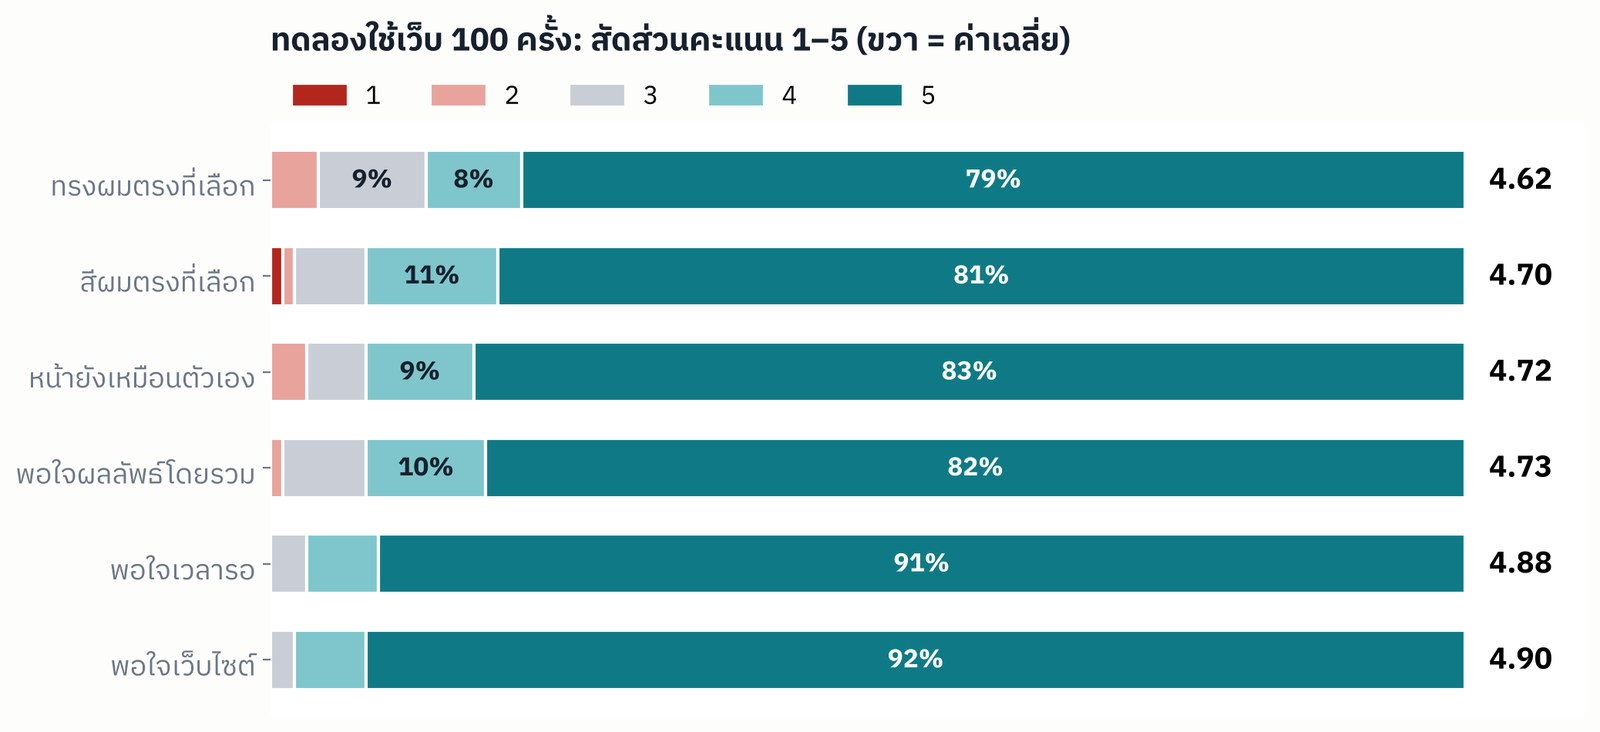
\includegraphics[width=\textwidth]{images/13_web_ratings.jpg}
\caption{สัดส่วนคะแนน 1--5}
\end{subfigure}
\hfill
\begin{subfigure}{0.41\textwidth}
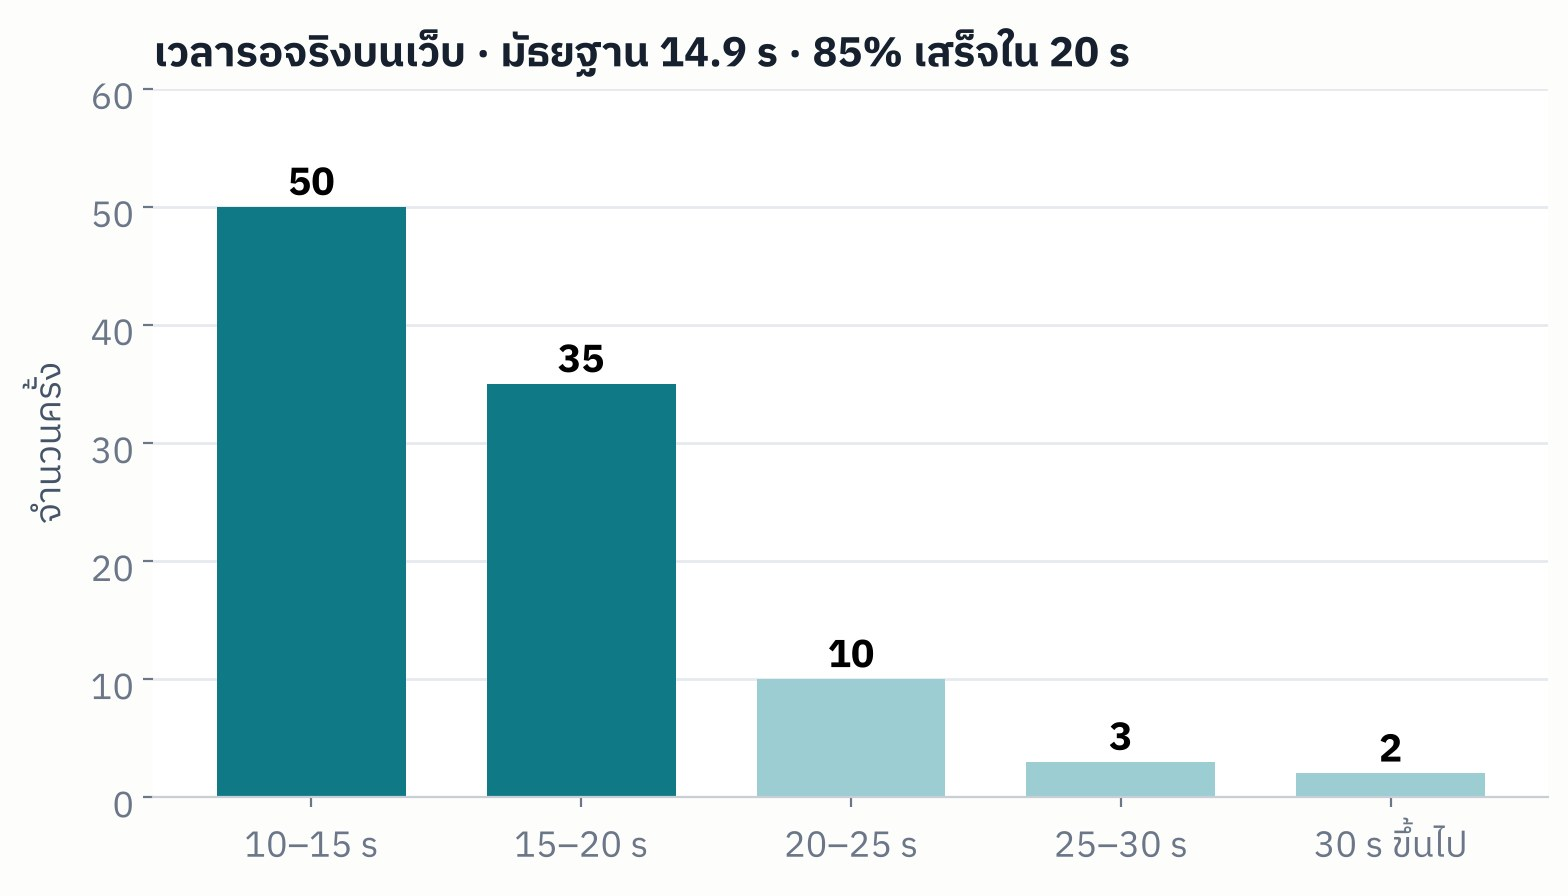
\includegraphics[width=\textwidth]{images/14_web_wait.jpg}
\caption{เวลารอจริง}
\end{subfigure}
\caption{ผลการทดลองใช้งานเว็บแอปพลิเคชัน 100 ครั้ง}
\label{fig:web}
\end{figure}

ผู้ใช้เขียนข้อเสนอแนะมา 4 ความเห็น ได้แก่ ``อยากให้ทรงผมดูเหมือนจริงขึ้นอีก''
``ผมมีความฟูกว่าปกติจึงดูไม่ค่อยตรงภาพอ้างอิง แต่โดยรวมเว็บใช้ง่ายและหน้าเว็บสวยงาม
ถ้ามีฟีเจอร์หวีผมจะดีมาก'' ``พื้นหลังดูแปลก'' และ ``ทรงผมดูไม่ค่อยเรียบเนียน แต่นอกนั้นทำได้ดี''
สามในสี่ความเห็นพูดถึงทรงผม ทั้งเรื่องความฟูและความเรียบ
ซึ่งตรงกับจุดอ่อนที่ผู้วิจัยทราบอยู่แล้ว เพราะส่วนที่ควบคุมทรงของ HFG ไม่ได้ถูกปรับจูน
ส่วนเรื่องพื้นหลังน่าจะมาจากขั้นเก็บพื้นหลังที่เติมรายละเอียดเข้าไป ซึ่งอาจมากเกินไปสำหรับบางภาพ

% -----------------------------------------------------------
\section{อภิปรายผล}
% -----------------------------------------------------------

\subsection{เหตุผลที่ปรับจูนเฉพาะโมดูล Color และ Refinement ของ HairFastGAN}

ตอนที่ผู้วิจัยรัน HairFastGAN ครั้งแรก พบว่าผมยังเป็นปื้นและสีไม่ตรงกับภาพอ้างอิง
ผู้วิจัยจึงลองปรับจูนทั้งโมเดลก่อน แต่ส่วนจัดทรง (Alignment) ไม่ดีขึ้น
เมื่อลองปรับเฉพาะโมดูล Color กับ Refinement สีกลับตรงภาพอ้างอิงมากขึ้น จึงเลือกปรับจูนเฉพาะสองโมดูลนี้
ในการทดลองช่วงแรกใช้ประมาณ 5 Epoch แล้วผลดีขึ้น จึงตั้งการฝึกจริงไว้ 30 Epoch

\subsection{ทรงผมของ Barbershop-FT แทบไม่เปลี่ยนหลังปรับจูน}

การเพิ่มจำนวน Epoch ของการปรับจูนน่าจะไม่ช่วยเรื่องทรงผม เพราะทรงผมของ Barbershop ถูกกำหนดในขั้นจัดรูป (Alignment)
ซึ่งค้นหารหัสแฝง (Latent) ใหม่ทุกภาพด้วยการวนซ้ำ และไม่ได้อยู่ในชั้นที่ปรับจูน
สิ่งที่น่าจะช่วยได้มากกว่าคือการเพิ่มจำนวนรอบค้นหาในขั้นนั้น ซึ่งต้องแลกกับเวลาที่นานขึ้น

\subsection{เหตุที่ Diffusion ทำให้ภาพดูดีขึ้นแต่ใบหน้าเหมือนเดิมน้อยลง}

ที่ผู้ใช้ให้คะแนนดีขึ้น น่าจะเป็นเพราะ Diffusion ทำให้เส้นผมชัดขึ้น
และใบหน้าสว่างใสขึ้นเล็กน้อย โดยไม่ได้เปลี่ยนไปจากเดิมมาก
ส่วนที่ผู้ใช้ให้คะแนนความเหมือนของใบหน้าน้อยลง (ตารางที่~\ref{tab:survey_pair})
ผู้วิจัยคิดว่าเป็นเพราะ Diffusion ปรับใบหน้าให้สว่างและเนียนเกินไป
ใบหน้าของผู้ใช้บางคนจึงเปลี่ยนไปมากจนดูไม่เหมือนรูปต้นฉบับ แม้คะแนนความพึงพอใจโดยรวมจะยังเพิ่มขึ้น

ในกรณีศึกษาเชิงตัวเลข 8 ชุดภาพ หลังผ่าน Diffusion ค่า ArcFace ลดลง 0.03--0.19 ทุกกรณี ซึ่งไปทางเดียวกับคะแนนผู้ใช้
ArcFace เทียบใบหน้ากับรูปต้นฉบับ ถ้าใบหน้าเปลี่ยนไปจากเดิม ค่าก็จะลดลง แม้การเปลี่ยนนั้นจะทำให้ภาพดูดีขึ้นก็ตาม
ส่วน MUSIQ ให้คะแนนคุณภาพภาพโดยไม่เทียบกับภาพเดิม และเปลี่ยนเพียง $-4.3$ ถึง $+1.9$ (เฉลี่ย $-1.84$ สำหรับ HFG และ $-0.06$ สำหรับ BS-FT)
ตัวเลขจึงบอกได้ว่าใบหน้าเปลี่ยน แต่บอกไม่ได้ว่าคนดูแล้วชอบขึ้นหรือไม่
ผู้วิจัยจึงใช้ตัวเลขดูว่ามีอะไรเสีย และใช้คะแนนจากผู้ใช้ดูว่าภาพดีขึ้นหรือไม่

\subsection{เหตุผลที่เลือก HairFastGAN B24 + Diffusion ไปใช้บนเว็บ}

ถ้าดูเพียงคุณภาพของภาพ Barbershop-FT + Diffusion ทำได้ดีที่สุด
เพราะได้คะแนนความสมจริงสูงสุด (3.83) และทรงผมตรงที่สุด (4.10)
แต่ใช้เวลาประมาณ 11 นาทีต่อภาพ ขณะที่ร้อยละ 84 ของคำตอบยอมรอได้ไม่เกิน 5 นาที
ถ้านำไปใช้บนเว็บ ผู้ใช้ส่วนใหญ่คงปิดหน้าเว็บไปก่อนได้ภาพ
และระบบนี้ยังได้คะแนนความเหมือนของใบหน้าต่ำสุด (3.22) ซึ่งสำคัญมากสำหรับระบบลองทรงผม
เพราะถ้าผลออกมาไม่เหมือนตัวเอง ผู้ใช้ก็ไม่รู้ว่าทรงนั้นเข้ากับตัวเองหรือไม่
HairFastGAN B24 + Diffusion ใช้เวลาประมาณ 13 วินาที ได้คะแนนความพึงพอใจสูงสุด (3.90)
และคะแนนความเหมือนของใบหน้าสูงกว่า Barbershop-FT + Diffusion อยู่ $+0.73$ คะแนน
ผู้วิจัยจึงเลือกระบบนี้ โดยยอมแลกกับความสมจริงที่ลดลงเล็กน้อย
ผลจากการใช้งานเว็บจริงที่ได้คะแนนความพอใจต่อเวลารอ 4.88 จาก 5 สนับสนุนการเลือกนี้

\subsection{สีผมของ HairFastGAN บนชุดทดสอบ}

หลังปรับจูน สีผิดของ HairFastGAN ลดจาก 13.03 เหลือ 8.99 แต่ช่วงความเชื่อมั่นยังแตะ 0 ($-8.19$ ถึง $+0.30$)
แปลว่ายังสรุปไม่ได้เต็มที่ว่าสีดีขึ้นในทุกกรณี
สาเหตุคือมี 3 จาก 10 ภาพที่สีแย่ลง เช่น test\_003 และชุดทดสอบมีเพียง 10 ชุด
ภาพที่แย่ลงเพียงไม่กี่ภาพจึงทำให้ผลแกว่งได้มาก
ต่างจาก ArcFace, MAE และ SSIM ที่ดีขึ้นครบทั้ง 10 ภาพ
ผู้วิจัยคิดว่าการปรับจูนช่วยเรื่องสีได้จริงในภาพรวม แต่ยังไม่นิ่งพอ
ถ้าจะยืนยันให้ชัด ต้องเพิ่มจำนวนชุดทดสอบ

\subsection{ความจำเป็นของด่าน 5 ด่าน}

ในการเลือก Checkpoint ถ้าดูเพียงคะแนนรวม Trial C และ D ของ Barbershop-FT
ได้คะแนนใกล้กับ Trial A มาก (0.856 และ 0.858 เทียบกับ 0.841)
แต่ทั้งสอง Trial มีค่า IoU ทรงผมต่ำกว่าตอนก่อนฝึกทุก Epoch แปลว่าทรงผมแย่ลงกว่าเดิม
ถ้าไม่มีด่าน ผู้วิจัยอาจเลือกโมเดลที่ทรงผมแย่ลงโดยไม่รู้ตัว
ด่านทั้ง 5 จึงช่วยกันไม่ให้เลือกโมเดลที่ดีขึ้นด้านหนึ่งแต่แย่ลงอีกด้านหนึ่ง

% -----------------------------------------------------------
\section{ข้อจำกัดที่พบ}
% -----------------------------------------------------------

ผู้วิจัยขอระบุข้อจำกัดของผลการทดลองไว้อย่างตรงไปตรงมา เพื่อให้ผู้อ่านตีความผลได้ถูกต้อง
ข้อแรกคือระบบต้องใช้ GPU (Graphics Processing Unit) ประสิทธิภาพสูง (ทดสอบบน A100 40 GB) จึงจะได้เวลาประมาณ 11--14 วินาทีต่อภาพ
บนเครื่องที่ช้ากว่านี้จะใช้เวลานานขึ้นมาก
ข้อที่สองคือข้อมูลมีขนาดเล็ก ชุดตรวจสอบมี 9 ชุด ชุดทดสอบมี 10 ชุด
และการวัดผลขั้น Diffusion ด้วยตัวเลขใช้เพียง 8 ชุดภาพต่อโมเดลกับ Seed เดียว
ค่าสีผิดจึงแกว่งมาก และมีบางภาพที่แย่ลงหลังปรับจูน เช่น ภาพ test\_003 ของ HFG
ข้อที่สามคือ Barbershop-FT บันทึกน้ำหนักไว้เพียง Epoch 0 และ 30 จึงเลือกได้จาก Epoch 30 เท่านั้น
ข้อที่สี่คือ IoU ทรงผมของทั้งสองโมเดลวัดกับทรงเป้าหมายที่มาจากโมดูล Shape ของ HairFastGAN
ซึ่งอาจเข้าข้าง HFG อยู่บ้าง เพราะเป็นทรงที่ HFG สร้างเอง
ข้อที่ห้าคือ Diffusion อาจทำให้สีผมและใบหน้าเปลี่ยนเล็กน้อย
และบริเวณที่ถูกแก้ไขขึ้นกับการแบ่งส่วนภาพ ถ้าหน้ากากตรวจไม่พบเส้นผมบางเส้น เส้นนั้นก็จะไม่ถูกขัดเกลา
ข้อสุดท้ายคือผู้ใช้ส่วนใหญ่ทั้งในการประเมินและบนเว็บมีอายุ 18--24 ปี
ผลจึงอาจไม่สะท้อนความเห็นของคนกลุ่มอายุอื่น

นอกจากนี้ ผลเชิงตัวเลขของ Diffusion เป็นกรณีศึกษา 8 ชุดภาพต่อโมเดลและ Seed เดียว
แม้จะใช้ HFG B24 และ BS-FT A30 ตัวเดียวกับในแบบสอบถาม แต่เป็นภาพคนละชุดกับที่ผู้ใช้ประเมิน
จึงไม่ควรสรุปขนาดผลของ Diffusion สำหรับทั้งชุดข้อมูล หรือโยงตัวเลขสองส่วนนี้เข้าหากันโดยตรง
ควรขยายการวัดให้ครอบคลุมทั้งชุดทดสอบ พร้อมรายงานค่าเฉลี่ยและความแปรปรวน
การวัดผลทีละขั้นเป็นการดูผลสะสม ไม่ใช่การทดลองตัดองค์ประกอบออกทีละส่วน (Ablation Study)
คำอธิบายสาเหตุเกี่ยวกับโมดูลต่าง ๆ และการที่ผู้ใช้ยอมแลกความเหมือนของใบหน้ากับรายละเอียดของผม จึงยังเป็นข้อสันนิษฐาน

ช่วงความเชื่อมั่นในเล่มนี้คำนวณแยกทีละการเปรียบเทียบ และยังไม่ได้ปรับแก้สำหรับการเปรียบเทียบหลายครั้ง (Multiple Comparisons)
จึงควรตีความเป็นหลักฐานเชิงสำรวจ โดยเฉพาะช่วงที่ขอบปัดเศษแล้วเป็นศูนย์
การตรวจข้อมูลซ้ำใช้ค่าแฮชของไฟล์ ซึ่งยืนยันได้ว่าไม่มีไฟล์ซ้ำข้ามชุดข้อมูล
แต่ไม่ได้ตรวจว่าบุคคลเดียวกันปรากฏในหลายชุดด้วยภาพคนละภาพหรือไม่
ด้านเวลา ค่าประมาณ 10 วินาทีของ HFG วัดครั้งเดียว รวมขั้นจัดตำแหน่งภาพแต่ไม่รวมการโหลดโมเดล
ส่วน 657 วินาทีของ Barbershop คือผลรวมเวลาคำนวณของขั้น $W^{+}$, $FS$, การจัดทรง การจัดสี และการผสม
ไม่รวมการโหลดโมเดล ส่วนเวลาของขั้น Diffusion เป็นค่าเฉลี่ยจาก 8 ชุดภาพในกรณีศึกษา
